\documentclass[a4paper,hidelinks,12pt]{article}
\usepackage[T2A]{fontenc}
\usepackage[utf8]{inputenc}
\usepackage[russian]{babel}
\usepackage{amsmath,graphicx}
\usepackage{indentfirst}
\usepackage{colortbl}
\usepackage{setspace}
\usepackage{float}
\usepackage{amssymb}
\usepackage{amsmath}
\usepackage{graphicx}
\usepackage{listings}
\usepackage{subcaption}
\usepackage{xcolor}
\usepackage{algorithm}
\usepackage{algpseudocode}
\usepackage{tabularx}
\RequirePackage{booktabs}
\definecolor{gray}{rgb}{0.4,0.4,0.4}
\definecolor{darkblue}{rgb}{0.0,0.0,0.6}
\definecolor{cyan}{rgb}{0.0,0.5,0.5}
\definecolor{maroon}{rgb}{0.5,0,0}
\definecolor{darkgreen}{rgb}{0,0.5,0}


\usepackage[left=3cm,right=1.5cm,top=2cm,bottom=2cm,bindingoffset=0cm]{geometry}
\setcounter{secnumdepth}{4}
\linespread{1.5}
\usepackage{xcolor}

\newenvironment{alphasection}{%
	\ifnum\alphainsection=1%
	\errhelp={Let other blocks end at the beginning of the next block.}
	\errmessage{Nested Alpha section not allowed}
	\fi%
	\setcounter{alphasect}{0}
	\def\alphainsection{1}
}{%
	\setcounter{alphasect}{0}
	\def\alphainsection{0}
}%


\begin {document}
\begin {titlepage}
\thispagestyle{empty}

\begin{center}
	\vspace{-1cm}
	
	
	%
	% No necessity to specify laboratory.
	%
	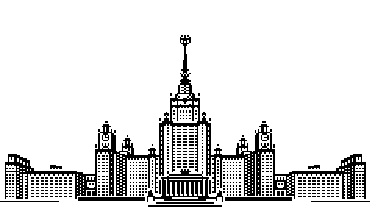
\includegraphics[width=0.5\textwidth]{msu}\\
	Московский Государственный Университет им. М.В. Ломоносова\\
	Факультет Вычислительной Математики и Кибернетики\\
	Кафедра Интеллектуальных Информационных Технологий\\
	
	\vspace{3cm}
	
	{\Large Майоров Николай Дмитриевич}
	
	\vspace{1cm}
	
	{\LARGE\bfseries Универсальные дифференцируемые представления объектов\\}
	
	\vspace{1cm}
	
	{ ВЫПУСКНАЯ КВАЛИФИКАЦИОННАЯ РАБОТА}
\end{center}

\vfill

\begin{flushright}
	\textbf {Научный руководитель:}\\
	к.ф.-м.н.\\
	В.А.Фролов\\
	\vspace{10mm}
\end{flushright}

\vfill

\begin{center}
	Москва, 2024
\end{center}

\end{titlepage}

\setcounter{page}{2}
\onehalfspacing

\begin{abstract}
Данная работа посвящена созданию нескольких дифференцируемых процедурных генераторов. Каждый из них способен получать объект своего класса по параметрам и матрицу производных выходных элементов по входным данным. Полученные генераторы используются в задаче трёхмерной реконструкции. В работе также представлена идея универсального дифференцируемого процедурного генератора, основанного на деревьях. Он может создавать модели вне зависимости от их класса, и также возвращает производные по параметрам. Генератор легко дополняется новыми элементами и масштабируется при необходимости. 
\end{abstract}

\newpage
\tableofcontents

\newpage
\section{Введение}
Индустрия компьютерных игр и кино – это сектор экономики, связанный с их продвижением, продажей и разработкой. Зародившись просто как необычное хобби группы увлечённых людей, в наши дни эта индустрия породила много специальностей, в которых задействованы тысячи людей. И развитие отрасли продолжается. А для заполнения виртуальных миров, создателям контента нужны разнообразные объекты. Каждая 3D модель, сделанная вручную, требует больших трудозатрат. Их можно создавать, используя процедурную генерацию, а можно восстанавливать существующие в реальности объекты.  
\par
В компьютерной графике существуют разнообразные представления объектов. Самое простое и часто используемое – полигональная сетка (меш). Используя её, можно задать любую поверхность с нужной точностью. Чем сложнее поверхность, тем больше полигонов необходимо использовать в сетке. Ещё одно распространённое представление объектов – функция расстояния со знаком (SDF). Она по координатам точки возвращает расстояние до поверхности объекта. С её помощью можно точно представить как трёхмерные, так и двухмерные объекты.
\par
Модель можно построить процедурно: объекты задаются при помощи параметров посредством процедурного генератора. Процедурный генератор – это функция, которая принимает на вход параметры и возвращает определённое представление объектов. Параметры могут задавать характеристики объекта, интуитивно понятные пользователю, например, размеры. Хранение таких моделей занимает существенно меньше памяти.
\par
В процессе работы реализованы процедурные дифференцируемые генераторы. Дифференцируемость генератора означает, что есть возможность узнать зависимость возвращаемого значения генератора от его параметров, то есть посчитать частную производную. Для различных представлений необходимо считать производные по-разному. Для полигональной сетки – производную позиции каждого узла сетки по параметрам. Для функции расстояния со знаком – производную расстояния по параметрам. Наличие у генератора производных позволяет оптимизировать его результат. Таким образом, появляется возможность решения обратной задачи – получение параметров для генератора по модели или её части. 
\par
Дифференцируемые представления объектов и дифференцируемые процедурные генераторы дают возможность получать модели, используя градиентные методы оптимизации. Если же генераторы будут ещё и универсальными, это может позволить реконструировать любые модели, не обращая внимания на вид или класс объекта. Написанные в рамках данной работы генераторы уже используются для восстановления объектов по одному изображению \cite{garifullin2023diff} \cite{garifullin2024single}.
\par
Идея универсального генератора заключается в том, что с его помощью можно создать любую модель. То есть, не нужно создавать принципиально новый генератор, если появилась необходимость в объектах нового класса. Но реконструкция с использованием такого генератора будет требовать более сложного алгоритма. 



\section{Постановка задачи}
Основная задача состояла в разработке дифференцируемых процедурных генераторов и, затем, универсального дифференцируемого процедурного генератора.
\par
Процедурный генератор должен по списку параметров длины n возвращать модель в одном из существующих представлений. В данном случае, возвращать либо полигональную сетку, либо функцию расстояния со знаком.
\par
Поскольку генератор дифференцируемый, в дополнение к модели он должен возвращать производные составляющих модели по входным параметрам.
\subsection{Цели работы}
%лучше как-то более чётко сформулировать, что ты хочешь предложить метод длля реализации процедурных генераторов принципиально-различных 3D объектов и поэтому двигаешься от простого к сложному:
Были поставлены следующие цели работы:
\begin{enumerate}
\item Разработать дифференцируемый процедурный генератор моделей 1-ого типа;
\item Разработать дифференцируемый процедурный генератор моделей 2-ого типа;
\item Интегрировать генераторы в программу 3D реконструкции;
\item Реализовать составляющие универсального дифференцируемого процедурного генератора;
\item Произвести экспериментальную оценку результатов реконструкции с использованием дифференцируемых процедурных генераторов.
\end{enumerate}
\newpage
\subsection{Формальная постановка задачи}
В работе созданы генераторы, использующие разные представления объектов:
\begin{enumerate}
\item Полигональные сетки:

Вход:
\begin{itemize}
    \item $Params \in \mathbb {R}^n$ - вектор длины $n$, набор числовых параметров для генерации;
    \item $Structure \in \mathbb {N}^m$ - вектор длины $m$, список, описывающий
структуру дерева процедурного генератора;
    \item $n \in \mathbb {N}$ - число параметров;
    \item $m \in \mathbb {N}$ - число узлов в дереве.
\end{itemize}
Выход:
\begin{itemize}
    \item $Mesh \in \mathbb {R}^{3 \cdot k}$ - массив длины $3 \cdot k$, полигональная сетка, модель полученная из параметров;
    \item $Jac \in \mathbb {R}^{(3 \cdot k) \times n}$ - матрица размера $3 
\cdot k \times n$, содержащая производные элементов полигональной сетки по входным параметрам;
    \item $k \in \mathbb {N}$ - число точек в сетке.
\end{itemize}
\item Функции расстояния со знаком:

Вход:
\begin{itemize}
    \item $Params \in \mathbb {R}^n$ - вектор длины $n$, набор числовых параметров для генерации;
    \item $Position \in \mathbb {R}^3$ - вектор длины $3$, позиция, в которой будет посчитан результат функции;
    \item $Structure \in \mathbb {N}^m$ - вектор длины $m$, список, описывающий
структуру дерева процедурного генератора;
    \item $n \in \mathbb {N}$ - число параметров;
    \item $m \in \mathbb {N}$ - число узлов в дереве.
\end{itemize}
Выход:
\begin{itemize}
    \item $Dist \in \mathbb {R}$ - действительное число, знаковое расстояние до поверхности модели, полученное по входным параметрам в заданной точке;
    \item $Jac \in \mathbb {R}^{1 \times (n+3)}$ - матрица размера $1 \times (n+3)$, содержащая производные дистанции по входным параметрам и входной позиции.
\end{itemize}
\end{enumerate}

\newpage

\section{Обзор литературы}
\subsection{Представления объектов}
В компьютерной графике существует большое количество представлений объектов, таких как: 
\begin{itemize}
    \item Полигональные сетки;
    \item Воксельные сетки;
    \item Функции расстояния;
    \item Облака точек;
    \item Процедурные представления;
    \item Неявные представления, и другие.
\end{itemize}
Представление объектов в виде полигональной сетки является наиболее распространённым. Оно позволяет легко переносить различные модели между многими приложениями для редактирования или использования, например Blender, AutoCAD, и многие многие другие. Достаточно просто можно добавить мелкие детали и изменить форму объекта. Также есть возможность применять эффективные алгоритмы их рендеринга. Но при этом существуют и недостатки. Так, оптимизация поверхности модели может быть сложной, из-за невыпуклости оптимизируемой функции, в особенности при наличии мелких деталей \cite{garifullin2023diff} \cite{garifullin2024single}. Чтобы попробовать решить возникшую проблему, можно использовать воксельные сетки \cite{lombardi2019neural} \cite{vicini2021non}. Они помогут упростить поиск экстремума. Но и этот способ представления сцены имеет свои минусы. Восстановление объектов с мелкими деталями сильно усложняется. В качестве альтернативы предыдущим представлениям можно рассмотреть облака точек.Этот способ позволяет создавать высококачественные реконструкции сцен \cite{yifan2019differentiable} \cite{ruckert2022adop}.
\par
На сегодняшний день нейронные сети являются одним из самых актуальных направлений в совершенно различных областях. И в данном обзоре, безусловно, нельзя обойтись без их упоминания. Тем более, что использование нейронных сетей на основе координат, или по другому – нейронные поля, даёт довольно интересные результаты \cite{mildenhall2021nerf} \cite{fridovich2022plenoxels} \cite{muller2022instant}. Нейронные поля обрабатывают сложные сцены за считанные секунды, при этом выдавая достаточно качественные результаты. Однако, часто, их бывает неудобно использовать. Это происходит из-за того, что на практике эти результаты необходимо преобразовать из неявного представления в полигональную сетку, что даёт некачественную и неоптимальную модель.  

\subsection{Процедурная генерация}

\par
Процедурное представление объектов отсылает к большой области – процедурной генерации. Процедурная генерация контента – это способ создания объектов совершенно разных классов, от простых предметов, до целых виртуальных миров, при помощи алгоритмов и функций \cite{hendrikx2013procedural} \cite{freiknecht2017survey}. Этой теме посвящено много разнообразных статей \cite{viana2019survey} \cite{de2011survey}. Кроме того, стоит упомянуть об обратной процедурной генерации, которая может быть использована для восстановления параметров модели \cite{stava2014inverse} \cite{guo2020inverse} \cite{garifullin2022fitting} \cite{garifullin2023diff} \cite{garifullin2024single}. Поскольку сложные процедурные генераторы часто являются необратимыми функциями, работы по этой теме, несмотря на их большое количество и многообразие, плохо обобщаются, и обычно сосредоточены на конкретных классах процедурных моделей.
\par
Процедурные генераторы могут быть созданы с использованием формальных грамматик \cite{urban1} \cite{sportelli2014probabilistic}. Также интересным, и даже более распространённым является использование так называемых систем Линденмайера (L-систем), которые являются специальным видом формальной грамматики \cite{marvie2005fl} \cite{guo2020inverse}. Такие генераторы описывают модель при помощи набора правил преобразований символов из <<алфавита>> и начального символа. С использованием таких методов был реализован обратный процедурный генератор, основанный на L-системах, о чём подробно изложенно в следующей работе \cite{vst2010inverse}. Он позволяет задать L-системой любое двухмерное векторное изображение, а также по входному векторному изображению получить L-систему и легко её модифицировать при необходимости.
\par
Интересной представляется возможность создания генераторов на основе деревьев или графов, например, как в этой статье \cite{gaillard2022automatic}. В ней представлен генератор в виде графа узлов, с элементами дифференцирования. Однако, эта реализация не предполагает использование генератора для оптимизации за пределами некоторой локальной области, что отличает её от генераторов, описанных в рамках данной квалификационной работы. 

\subsection{Реконструкция трёхмерных моделей}

\par
Дифференцируемые генераторы создавались с целью использования их в задаче реконструкции трёхмерных объектов по одному изображению. Эта задача, на сегодняшний день, остается очень сложной, в первую очередь потому, что она является существенно некорректной. Очевидно, что на одном изображении видна только часть объекта, а для восстановления невидимых частей необходимо использовать дополнительные знания о структуре реконструируемого объекта. По этой причине методы машинного обучения являются самой распространенной группой методов для решения этой задачи. Эти методы используют различные представления сцены, такие как полигональные сетки (меши) \cite{wang2018pixel2mesh} \cite{nie2020total3dunderstanding} \cite{ye2021shelf}, воксельные сетки \cite{choy20163d} \cite{popov2020corenet}, облака точек \cite{fan2017point} \cite{chen2021unsupervised} или неявные функции \cite{chen2019learning}. Важно отметить, что эти методы обучаются и оцениваются на одних и тех же классах объектов и их применение к другим классам требует повторного обучения и наличия достаточно большой выборки 3D-моделей соответствующего типа. Недавняя работа \cite{tatarchenko2019single} показала, что такие подходы к реконструкции, в первую очередь, выполняют распознавание типа объекта, а не его реконструкцию и повышение качества результата их работы сильно затруднительно.
\par
Также стоит обратить внимание на несколько работ, реализующих восстановление 3D-модели по одному изображению, не ограничивая категорию объекта \cite{zhang2018learning} \cite{yang2022zeromesh}, что, в свою очередь, приводит к более низкому качеству моделей тех классов, которые не присутствовали в обучающей выборке.\\
\par
%Поскольку сложные процедурные генераторы часто являются необратимыми функциями, работы по этой теме, несмотря на их большое количество и многообразие, плохо обобщаются, и обычно сосредоточены на конкретных классах процедурных моделей.
Работы, связанные с процедурными генераторами и с обратной процедурной генерацией, в большинстве своём направлены на решение какой-то конкретной узкой задачи и плохо обобщаются. В то время, как эта работа посвящена созданию универсального дифференцируемого процедурного генератора, который планируется использовать для решения задачи 3D реконструкции без концентрации на конкретном классе объектов, рассматривая данную проблему значительно шире.




\section{Предложенные методы}
\subsection{Генераторы посуды и зданий}
\subsubsection{Подсчёт производных}
Дифференцируемый процедурный генератор отличается от обычного тем, что помимо созданного с помощью параметров объекта, он должен вернуть матрицу производных, в которой описывается зависимость всех выходных элементов от входных не дискретных параметров. Эта матрица может использоваться в алгоритмах реконструкции для расчёта производных функции потерь по параметрам \cite{garifullin2023diff} \cite{garifullin2024single}:
\par
$$\frac{\partial Loss} {\partial P} = \frac{\partial Loss} {\partial Pos} \cdot \frac{\partial Pos} {\partial P}$$
\par
Стоит заметить, что в большом количестве нетривиальных процедурных генераторов существуют дискретные зависимости, например, количество окон у здания, или наличие ручки у чашки. Для подбора этих параметров не получится использовать производные, и придётся искать другие подходящие алгоритмы, такие как, например, меметический алгоритм (memetic algorithm) \cite{garifullin2023diff} \cite{garifullin2024single}.
\subsubsection{Процедурный генератор посуды}
Первый из разработанных дифференцируемых процедурных генераторов – процедурный генератор посуды. Он является примером простого генератора, близкого в своем поведении к дифференцируемой функции, и имеет всего один дискретный параметр. Все остальные параметры у него вещественные. 
\par
Алгоритм создания полигональной сетки выглядит следующим образом:
\begin{itemize}
    \item Создаётся ломанная линия – сплайн по конечному числу параметров, имеющая координаты углов линии: $(0, 0), (x_1, 0), (x_2, 1) … (x_n, n-1)$;
    \item Линия загибается таким образом, чтобы получилась замкнутая петля определённой ширины, которая задаётся в параметрах;
    \item Эта линия вращается вокруг оси OY конечное количество раз, создавая дискретное тело вращения, и для каждой пары линий создаются треугольники в углах линий, которые добавляются в полигональную сетку;
    \item Если соответствующий дискретный параметр не равен 0, то создаётся правильный многоугольник, который несколько раз проворачивается на постоянный угол относительно центра, и отодвигается от центра на расстояние, заданное в параметрах для каждого поворота отдельно. Далее для каждой пары соседних многоугольников вновь создаются треугольники, соединяющие углы, и записанные в итоге в полигональную сетку.
\end{itemize}

\begin{figure}[H]
\begin{center}
	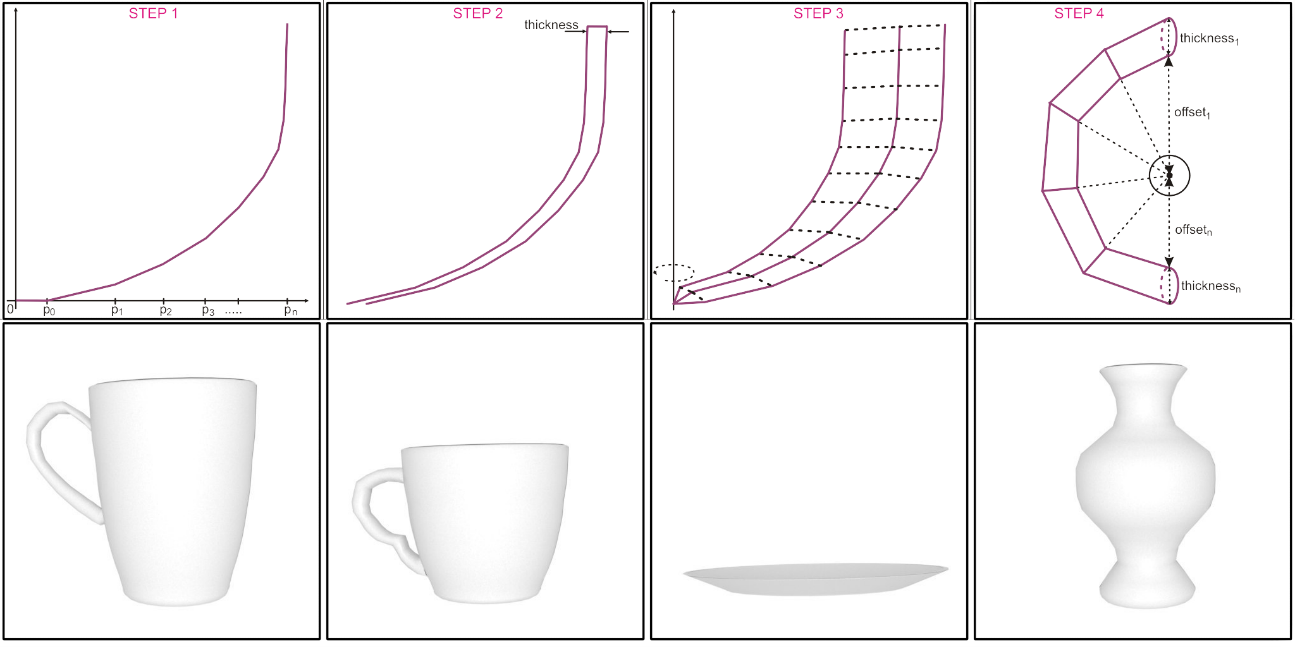
\includegraphics[width=15 cm]{algorithm.png}
	\caption{Верхний ряд: этапы генерации. Слева направо: 1) Создание сплайна из вектора вертикальных смещений. 2) Преобразование для создания замкнутого сплайна с заданной толщиной. 3) Вращение. 4) (Необязательно) Создание ручки из сплайна окружности и вектора смещений. Количество точек в сплайнах может быть изменено для получения различных уровней детализации на основе одного и того же набора параметров. Нижний ряд: примеры сгенерированных объектов. Слева направо: 1) Кружка 2) Чайная чашка 3) Тарелка 4) Ваза.}
 	\label{fig_alg}
\end{center}
\end{figure}

\par
Для поиска производных использовалась библиотека автоматического дифференцирования CppAD \cite{bell2012cppad}, которая позволяет получать требуемые производные из вычислительного графа, не вычисляя их явно внутри кода. 
\subsubsection{Процедурный генератор зданий}
Следующий реализованный генератор – генератор панельных зданий. В нём существенно больше дискретных параметров, отвечающих за количество этажей и подъездов и т.д. При этом он также обладает и вещественными параметрами, по которым возможно автоматическое дифференцирование. При создании полигональной сетки каждый элемент здания создаётся отдельно и добавляется в общий массив полигонов.
\begin{itemize}
    \item Стены с одной из сторон;
    \item Окна для каждой из стен;
    \item Стены с оставшихся сторон;
    \item Окна и двери для вновь созданных стен;
    \item Балконы для каждого уже созданного окна;
    \item Крыша, и прочие мелкие детали.
\end{itemize}

\begin{figure}[H]
\begin{center}
	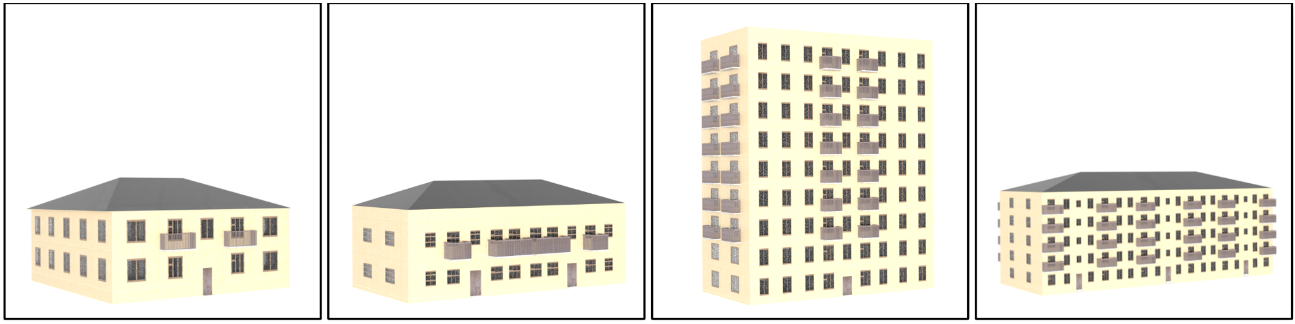
\includegraphics[width=15 cm]{houses_gen.png}
	\caption{Примеры созданных генератором зданий.}
 	\label{fig_house}
\end{center}
\end{figure}

\par
Для поиска производных по не дискретным параметрам в этом генераторе также использовалась библиотека CppAD \cite{bell2012cppad}.

\subsection{Универсальные генераторы}
\subsubsection{Структура универсального генератора}
Для реализации универсального генератора было написано дерево из узлов, в которых создавались примитивные модели, в дальнейшем модифицированные. Были реализованы узлы, создающие два типа моделей: полигональные сетки и функции расстояния со знаком. В процессе работы над универсальным генератором предпочтение было отдано реализации с использованием второго представления, так как это позволяло осуществлять более сложные взаимодействия между несколькими примитивами и упрощало расчёты, связанные с производными.
\par
Узлы имеют функцию, которая выдаёт в качестве результата модель. У каждого узла разное количество параметров, от которых зависит результат функции расчёта модели. Также узлы имеют некоторое количество дочерних узлов (обычно 0 – 2, но может быть и более), от которых тоже зависит результат. Один из узлов дерева считается корневым: с него начинается расчёт модели, которую должен создать генератор. Каждый узел принимает на вход также указатели на массивы частных производных $\frac{\partial Dist} {\partial Pos}$ и $\frac{\partial Dist} {\partial Params}$ и вычисляет их, если указатели не нулевые. Более подробно производные будут описаны в соответствующем разделе.
\subsubsection{Виды узлов в дереве генератора}
Дерево генератора состоит из узлов нескольких типов. Основные из них это:
\begin{itemize}
    \item Узлы примитивов;
    \item Узлы преобразований;
    \item Узлы комбинаций.
\end{itemize}
Есть и другие, например, сложные узлы, но про них будет написано ниже. На рисунке ~\ref{fig_nodes} показаны виды узлов, и их вложенность.
\par
Узлы примитивов – это те узлы, в которых высчитывается непосредственно некоторая примитивная модель от каких-то параметров. Они не зависят ни от каких других узлов, и, соответственно, не имеют дочерних узлов. Примеры узлов примитивов: узел шара, узел куба, узел цилиндра.
\par
Узлы преобразований – это узлы, в которых происходит изменение одной модели, полученной из дочернего узла. Примеры узлов преобразований: узел масштабирования, узел сдвига, узел поворота.
\par
Узлы комбинаций – те, в которых две других модели дают одну модель по каким-то правилам. Они зависят от двух дочерних узлов. Примеры подобных узлов: узел объединения, узел пересечения, узел вычитания.
\par
Для каждого узла известно количество его дочерних узлов, и в связи с этим возможно однозначно представить дерево процедурного генератора как список узлов (например, в порядке обхода дерева: корень – левый узел – правый узел).

\begin{figure}[H]
\begin{center}
	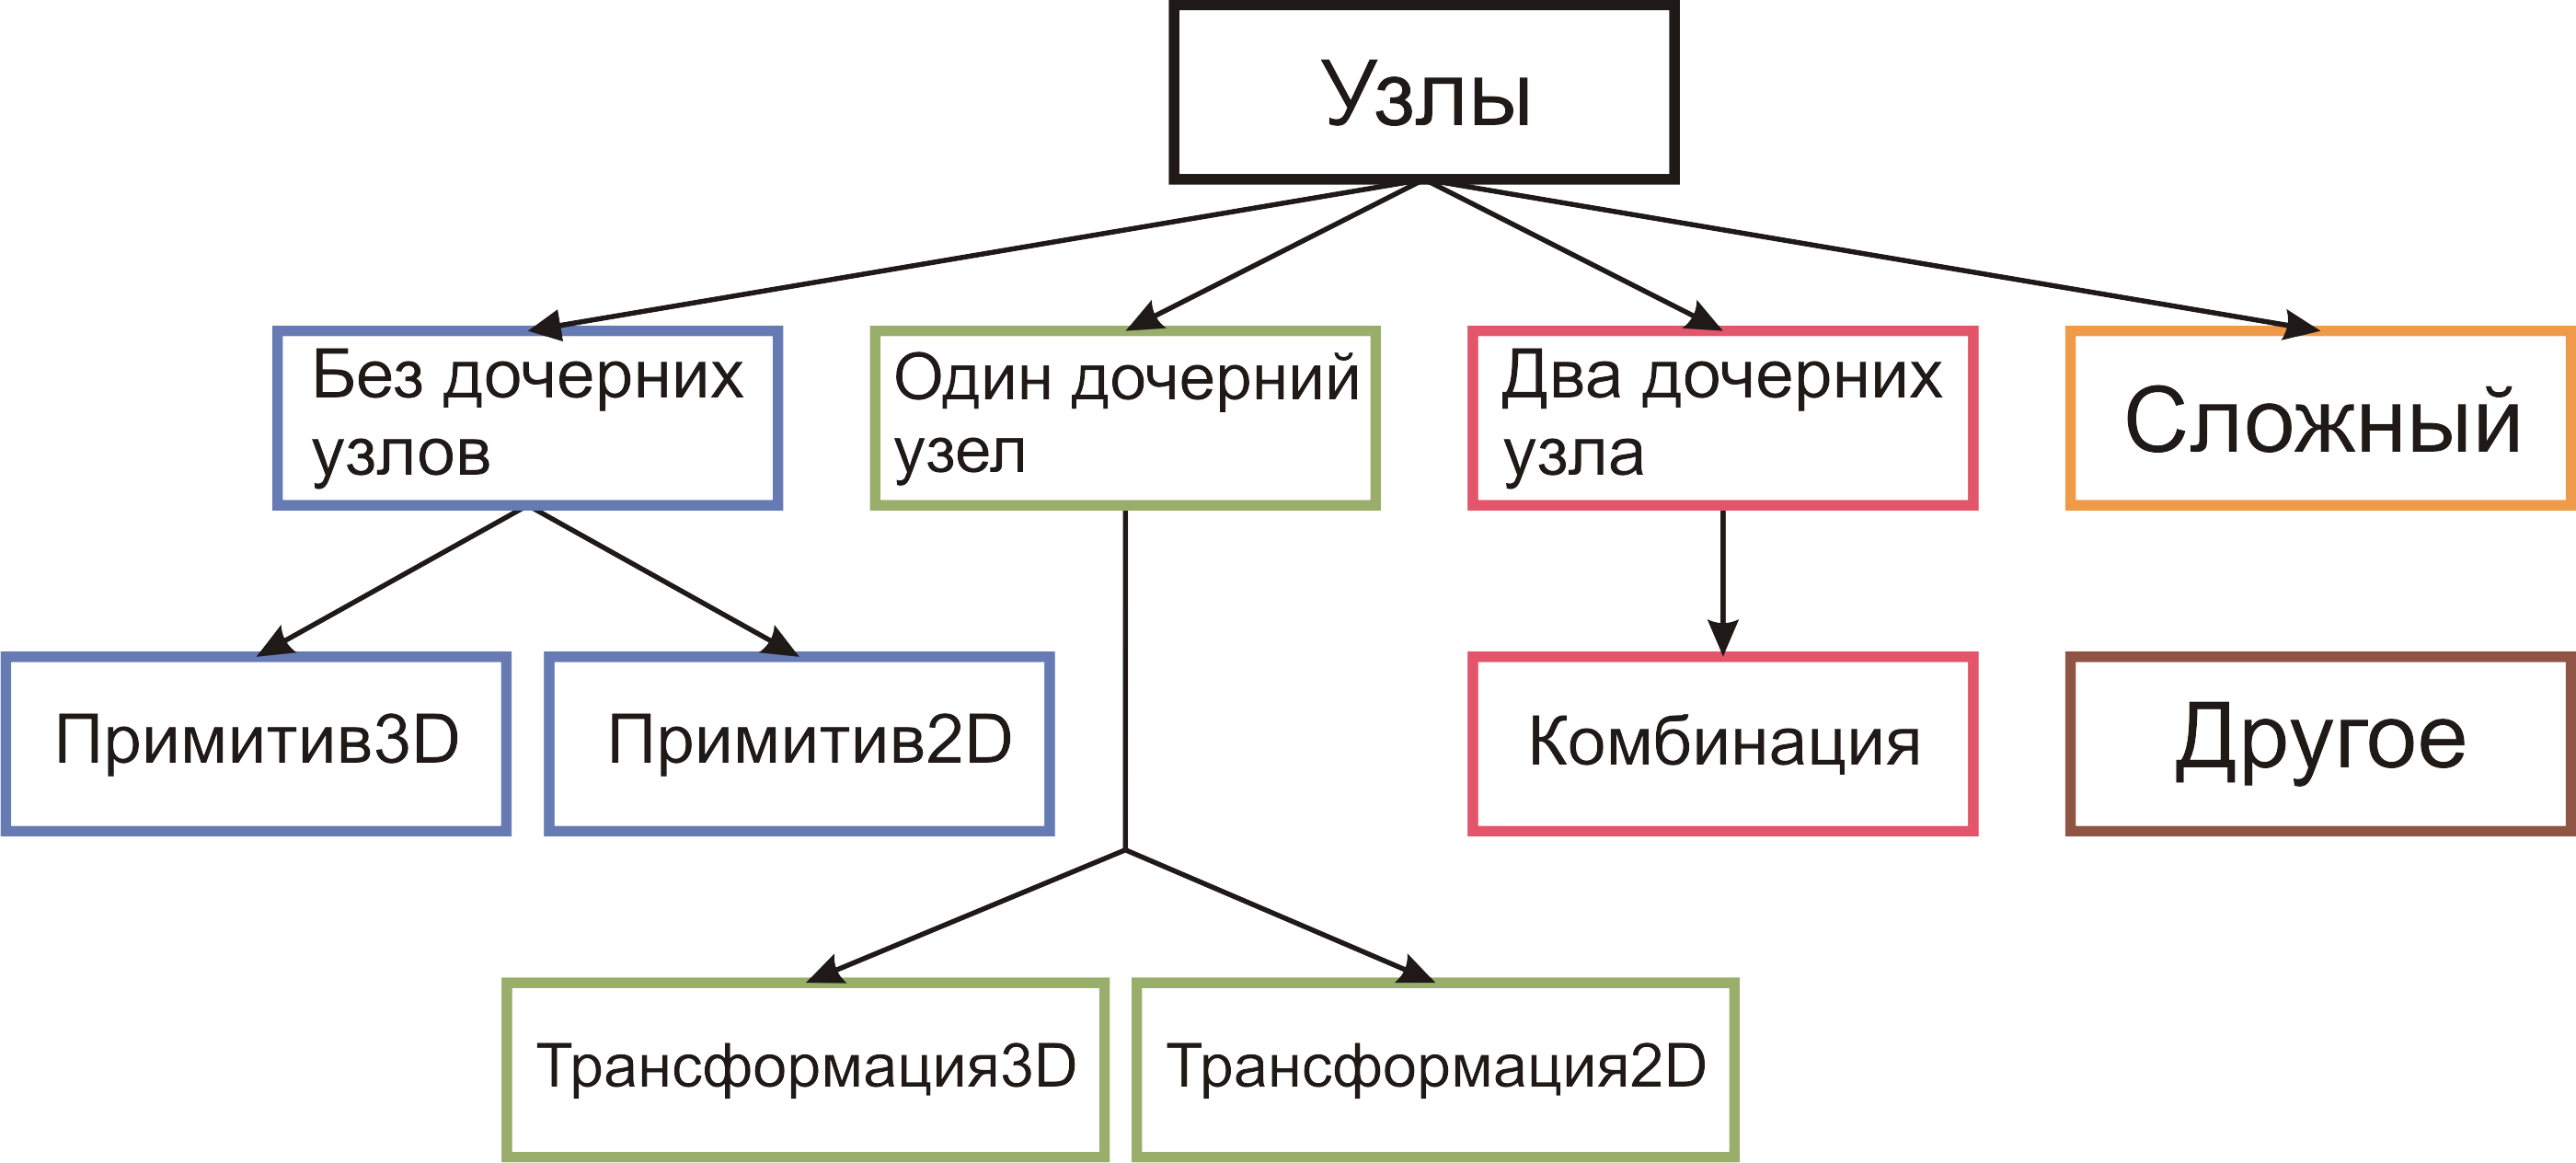
\includegraphics[width=15 cm]{Graphic_nodes_rus.png}
	\caption{Виды узлов и их вложенность.}
 	\label{fig_nodes}
\end{center}
\end{figure}

\subsubsection{Подсчёт производных в узлах}
Для подсчёта производных в дереве генератора необходимо посчитать их в каждом из узлов, в зависимости от входных параметров, и выходных данных дочерних узлов, то есть от представления объекта и матрицы производных, выданных каждым из дочерних узлов.
\par
Далее представлена формула подсчёта производных для узла, с n дочерними узлами, каждый из которых зависит от $k_i$ параметров. Все параметры считаются независимыми друг от друга.
\par
$$R = M \cdot U | N$$
В этом уравнении, операция $\cdot$ является матричным умножением, а операция $|$ конкатенацией двух матриц;
\begin{equation*}
R = \left(
\begin{array}{ccccc}
\frac{\partial new_1} {\partial P_{1,1}} & \ldots & \frac{\partial new_1} {\partial P_{1,k_1}} & \ldots & \frac{\partial new_1} {\partial P_{n+1,k_{n+1}}}\\
\vdots & \ddots & \vdots & \ddots & \vdots\\
\frac{\partial new_m} {\partial P_{1,1}} & \ldots & \frac{\partial new_m} {\partial P_{1,k_1}} & \ldots & \frac{\partial new_m} {\partial P_{n+1,k_{n+1}}}
\end{array}
\right)
\end{equation*}
Матрица $R$ содержит результат, то есть производные выходной модели по всем параметрам;
\begin{equation*}
M = \left(
\begin{array}{ccccc}
\frac{\partial new_1} {\partial old_{1,1}} & \ldots & \frac{\partial new_1} {\partial old_{1,m_1}} & \ldots & \frac{\partial new_1} {\partial old_{n,m_n}}\\
\vdots & \ddots & \vdots & \ddots & \vdots\\
\frac{\partial new_m} {\partial old_{1,1}} & \ldots & \frac{\partial new_m} {\partial old_{1,m_1}} & \ldots & \frac{\partial new_m} {\partial old_{n,m_n}}
\end{array}
\right)
\end{equation*}
Матрица $M$ содержит зависимости новой модели от дочерних, то есть производные элементов выходной модели по элементам всех входных моделей;
\begin{equation*}
U = \left(
\begin{array}{ccccc}
\frac{\partial old_{1,1}} {\partial P_{1,1}} & \ldots & \frac{\partial old_{1,1}} {\partial P_{1,k_1}} & \ldots & \frac{\partial old_{1,1}} {\partial P_{n+1,k_{n+1}}}\\
\vdots & \ddots & \vdots & \ddots & \vdots\\
\frac{\partial old_{1,m_1}} {\partial P_{1,1}} & \ldots & \frac{\partial old_{1,m_1}} {\partial P_{1,k_1}} & \ldots & \frac{\partial old_{1,m_1}} {\partial P_{n+1,k_{n+1}}}\\
\vdots & \ddots & \vdots & \ddots & \vdots\\
\frac{\partial old_{n,m_n}} {\partial P_{1,1}} & \ldots & \frac{\partial old_{n,m_n}} {\partial P_{1,k_1}} & \ldots & \frac{\partial old_{n,m_n}} {\partial P_{n+1,k_{n+1}}}
\end{array}
\right)
\end{equation*}
Матрица $U$ содержит зависимости всех дочерних моделей от всех старых параметров, то есть производные элементов всех входных моделей по параметрам, от которых они зависят;
\begin{equation*}
N = \left(
\begin{array}{ccc}
\frac{\partial new_1} {\partial P_{n+1,1}} & \ldots & \frac{\partial new_1} {\partial P_{n+1,k_{n+1}}}\\
\vdots & \ddots & \vdots\\
\frac{\partial new_m} {\partial P_{n+1,1}} & \ldots & \frac{\partial new_m} {\partial P_{n+1,k_{n+1}}}
\end{array}
\right)
\end{equation*}
Матрица $N$ содержит зависимости полученной модели от новых параметров, то есть производные элементов выходной модели по параметрам, от которых не зависят дочерние модели.

\begin{figure}[H]
\begin{center}
	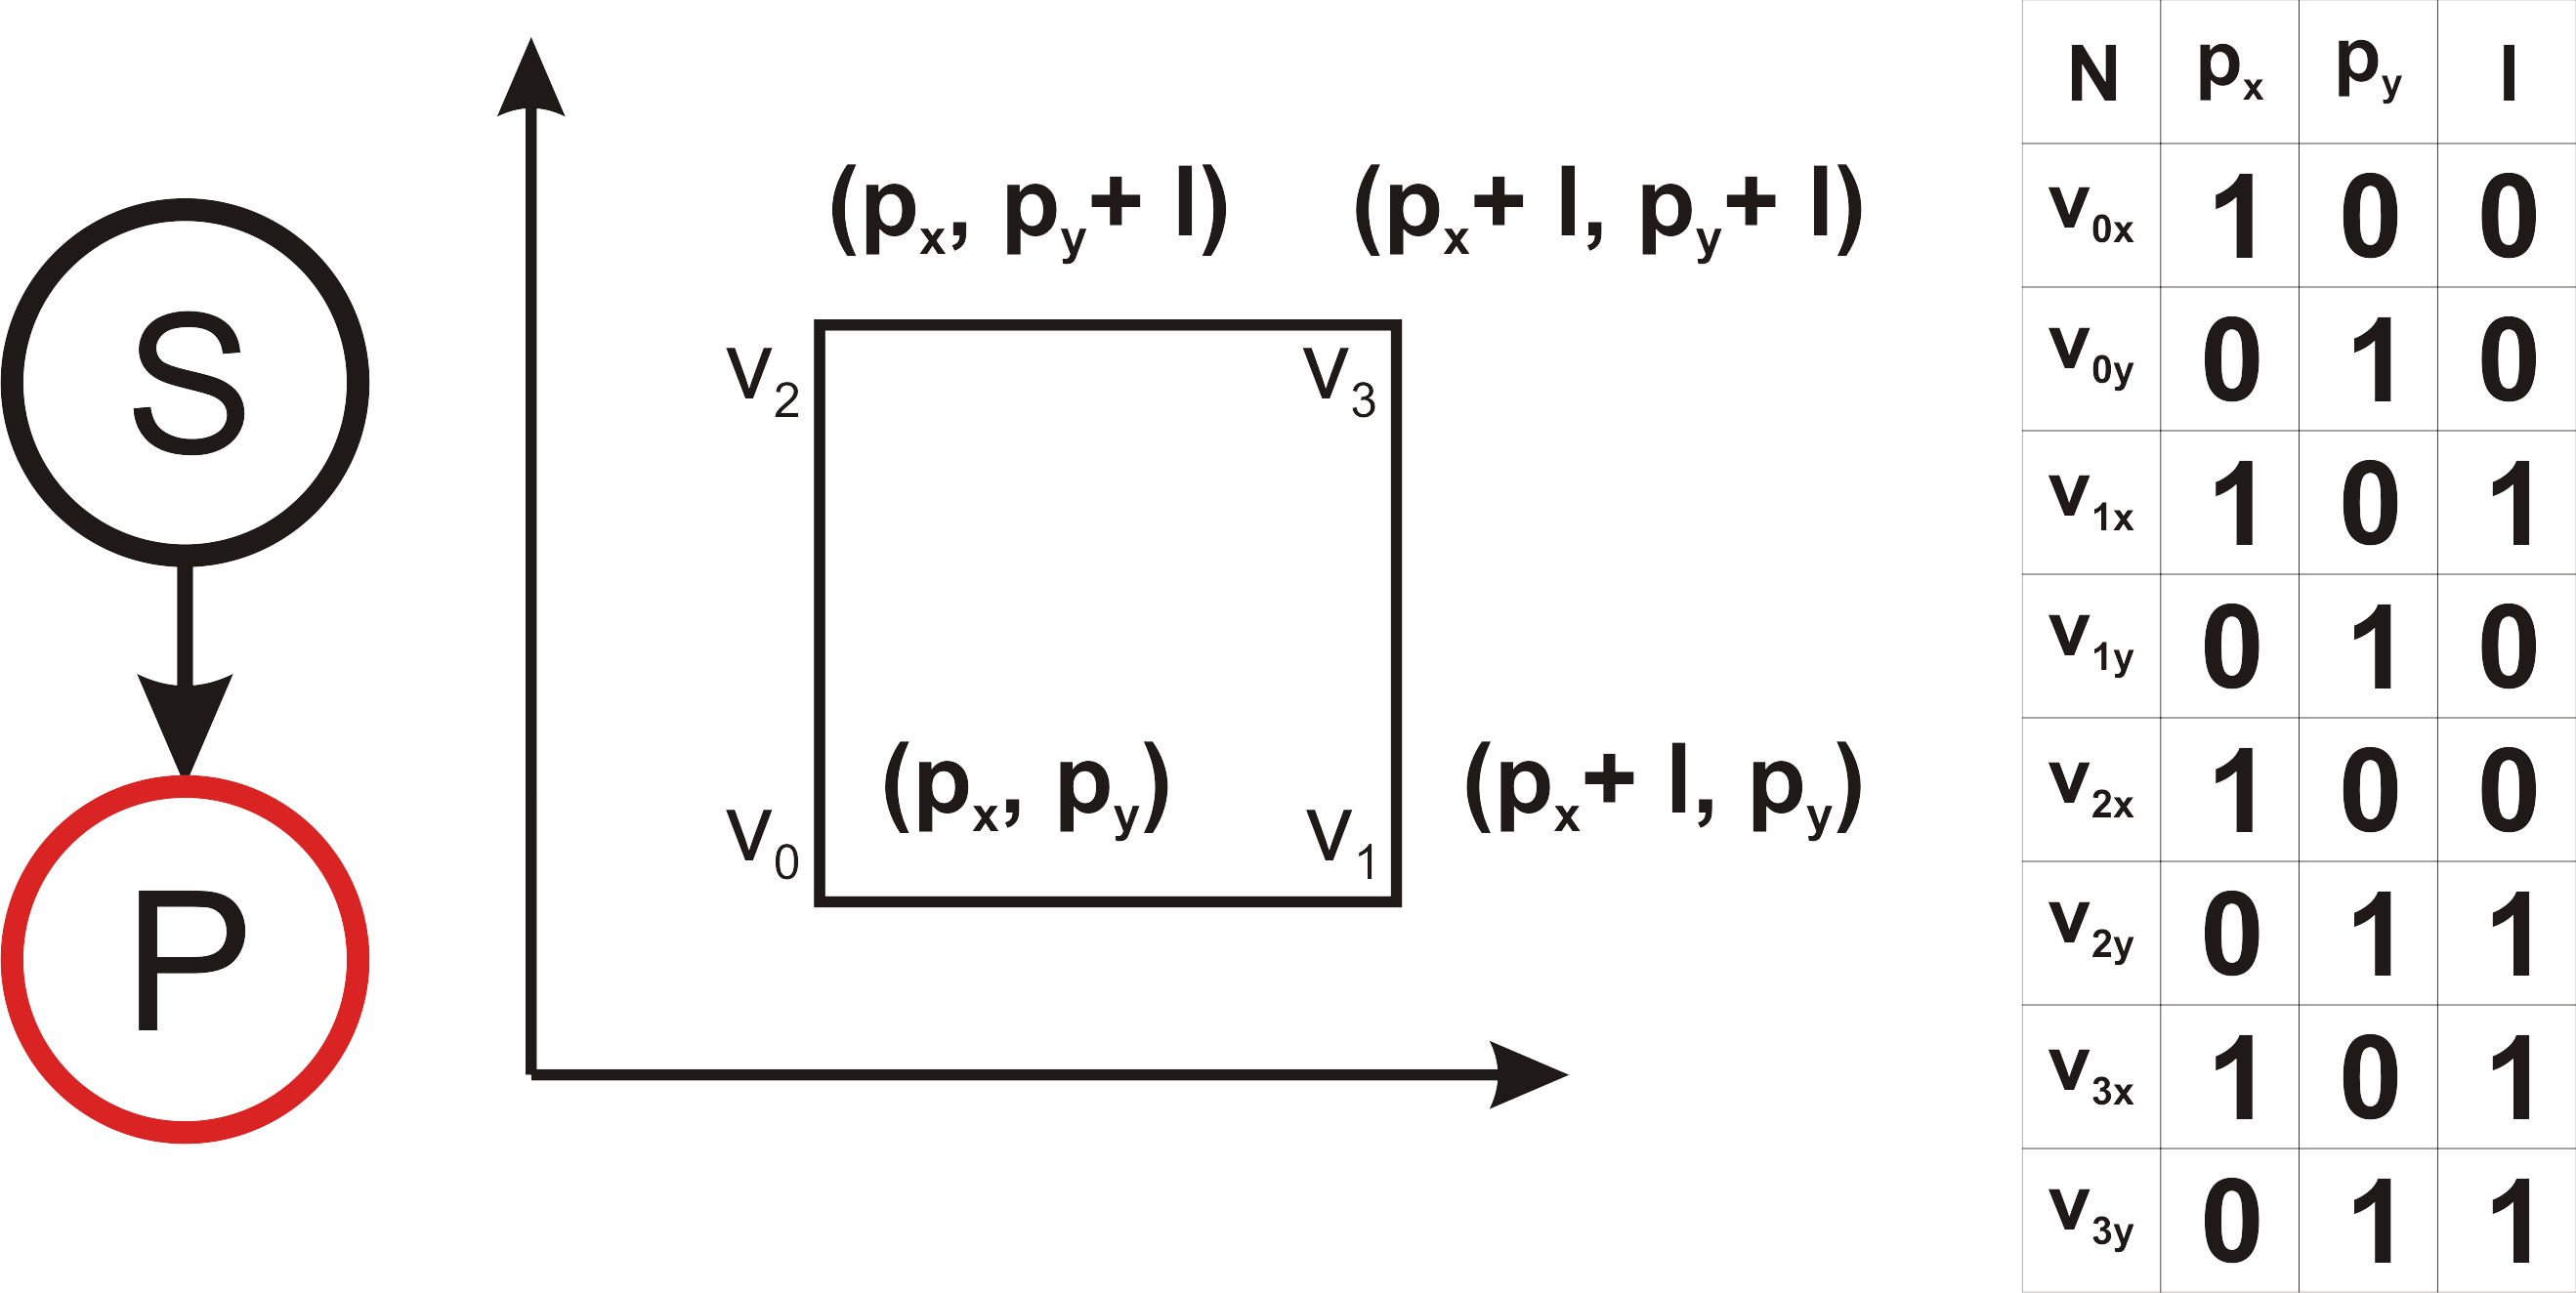
\includegraphics[width=15 cm]{primer1.png}
	\caption{Вычисления матрицы производных в узле примитива.}
 	\label{fig_p_1}
\end{center}
\end{figure}

\par
В качестве примера выше изложенного, можно предложить рассмотреть простое дерево, состоящее из двух узлов. На изображении~\ref{fig_p_1} находится первый узел, который создаёт квадрат заданного размера $l$ с нижним левым углом в заданной координате $p$. На изображении~\ref{fig_p_2} представленны вычисления в узле масштабирования в $s_x$ раз по оси x, и в $s_y$ по оси y. В формуле узла примитива матрицы $M$ и $U$ будут пустыми, по причине отсутствия дочерних узлов. Матрица $N$ будет иметь размер содержать зависимости восьми координат углов квадрата от трёх входных параметров. Итоговая матрица $R$ в этом узле будет совпадать с матрицей $N$. Затем необходимо посчитать матрицу зависимостей уже в узле преобразований. Матрица $M$ будет содержать зависимость новых координат углов квадрата от старых координат. Поскольку каждая координата угла меняется по формуле: $v'_i=v_i*s$, то и матрица $M$ будет выглядеть как диагональная матрица, содержащая на диагонали $s_x$ и $s_y$. Матрица $U$ будет совпадать с итоговой матрицей в узле примитива из-за того, что дочерний узел один. $N$, в свою очередь, содержит зависимость изменённых углов по новым переменным. В результате каждая строка матрицы $U$ увеличится в $s_x$ или $s_y$ раз, и к ней будет приписана новая матрица $N$, откуда и получается матрица зависимостей $R$ в узле преобразований.

\begin{figure}[H]
\begin{center}
	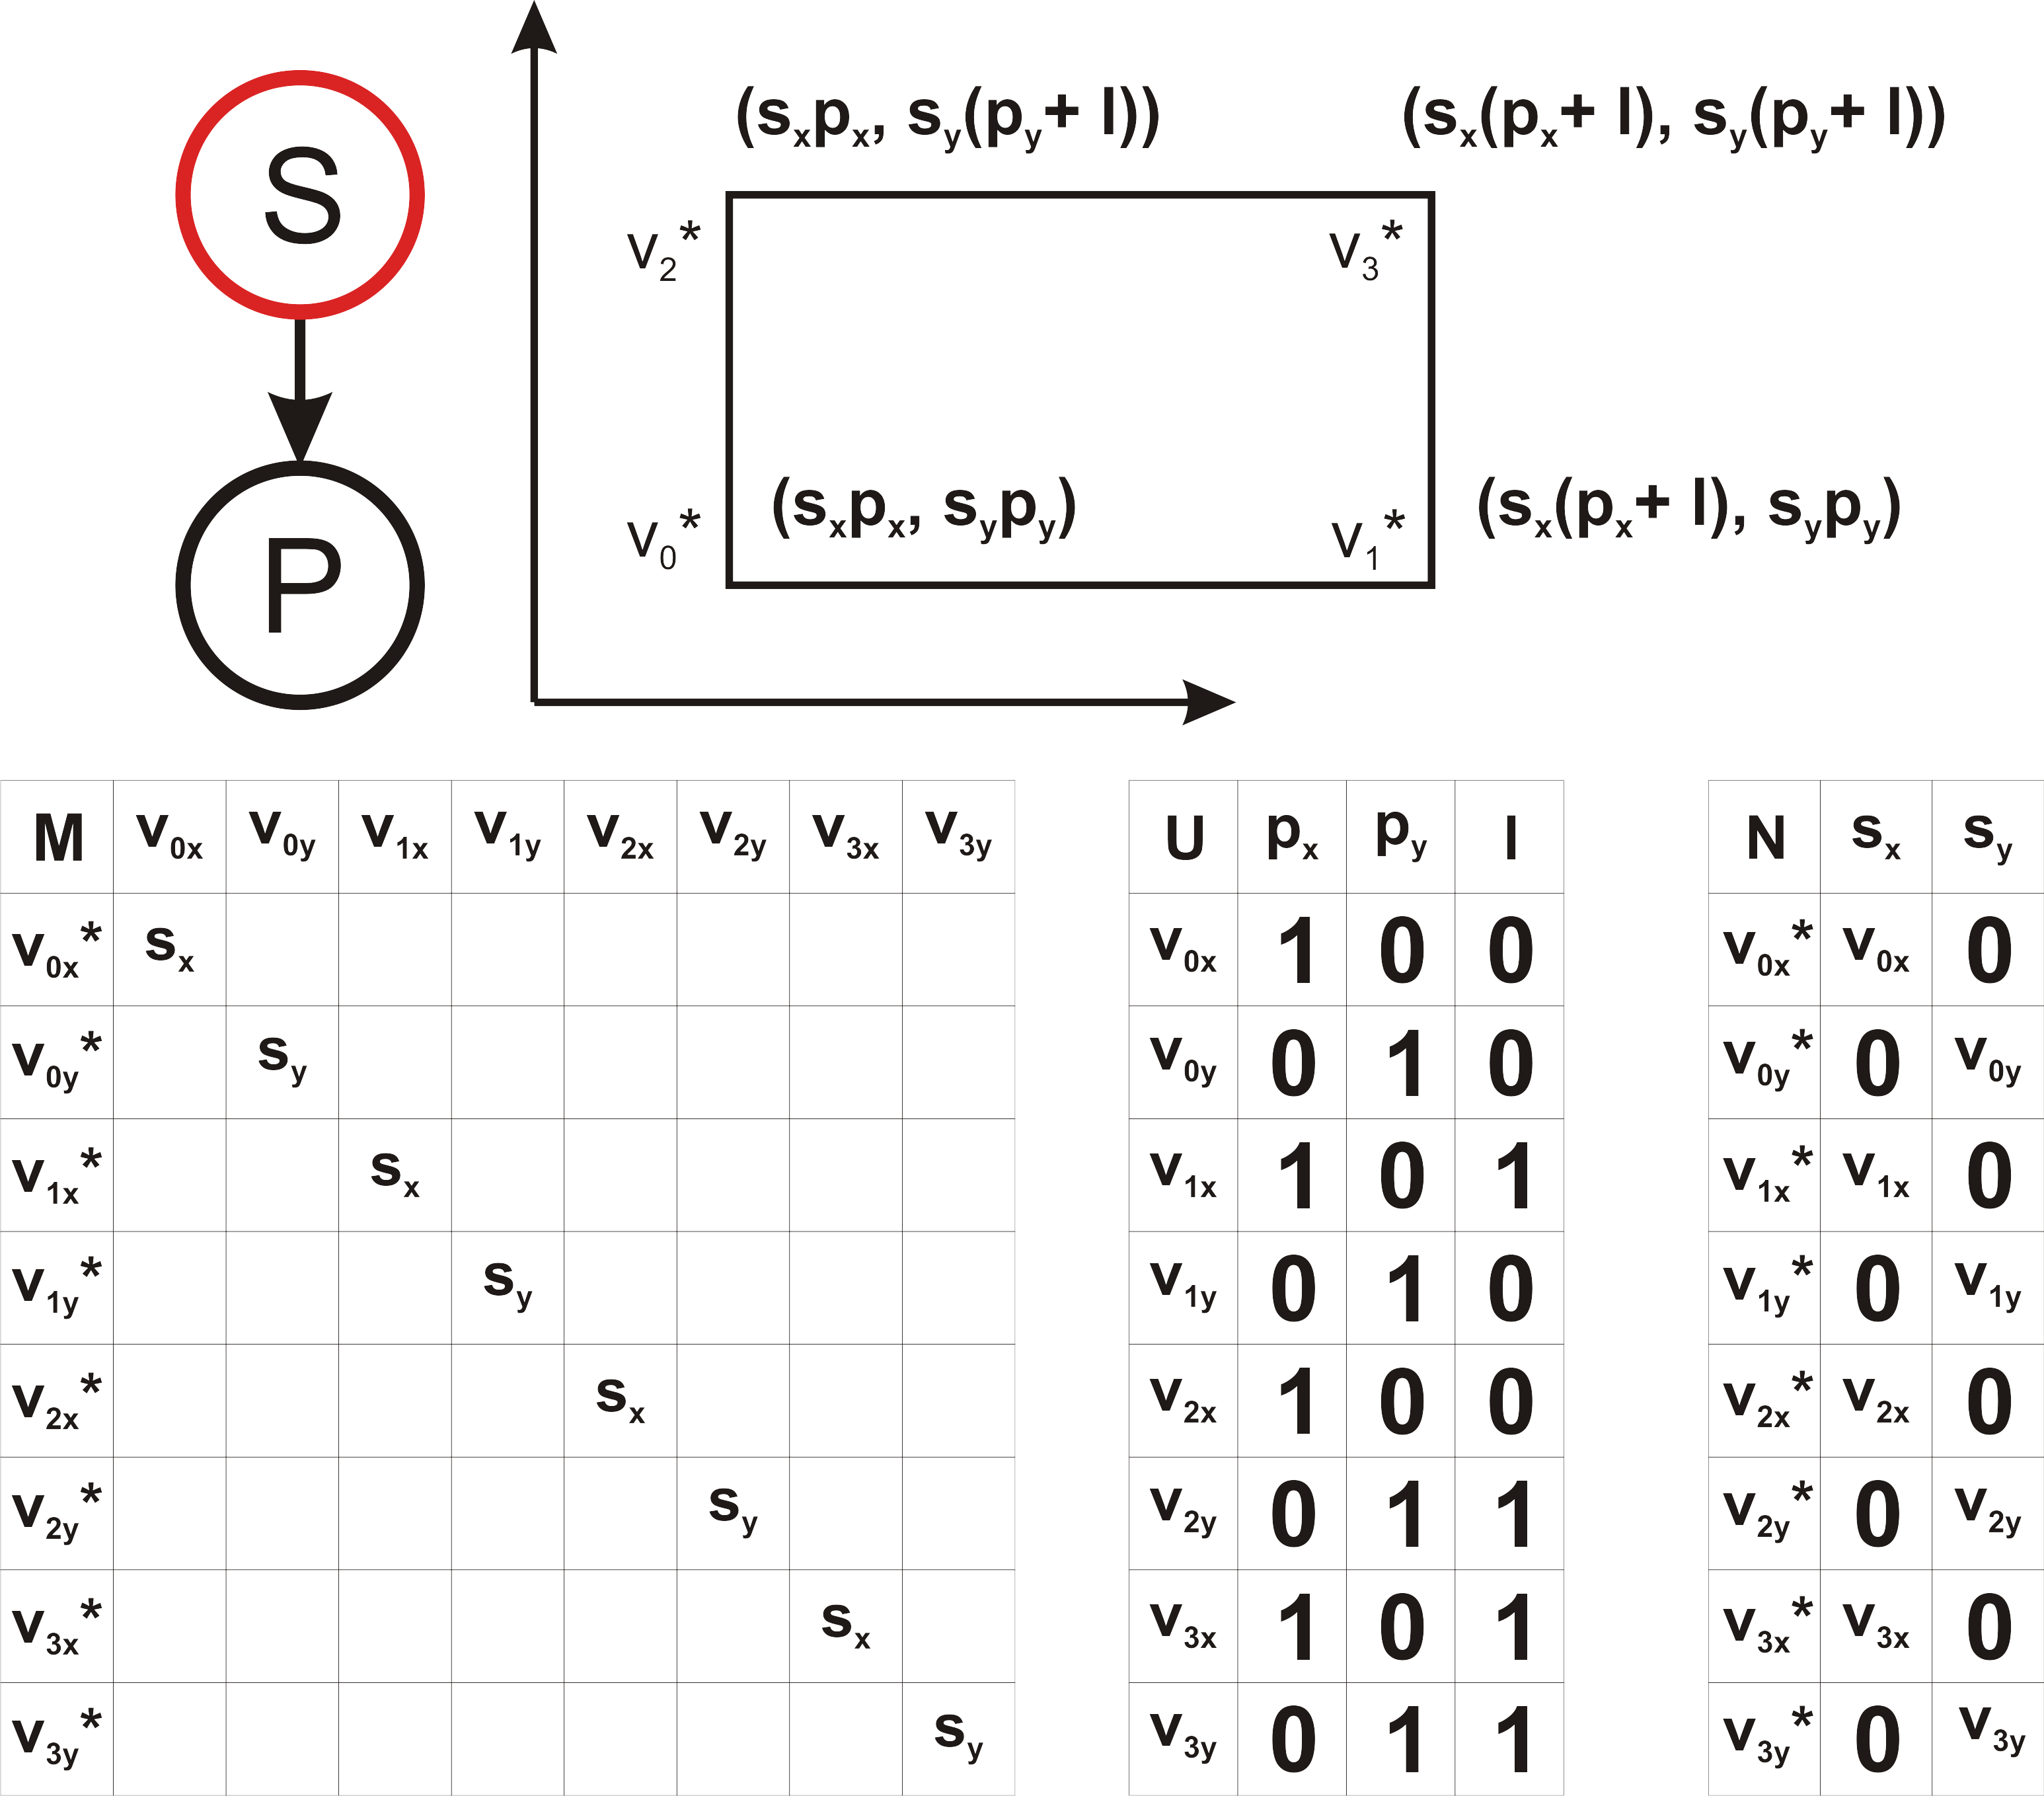
\includegraphics[width=15 cm]{primer2.png}
	\caption{Вычисления матрицы производных в узле преобразований.}
 	\label{fig_p_2}
\end{center}
\end{figure}

\par
Перемножение матриц – это затратная операция, что очень сильно может сказаться на скорости расчёта матрицы производных. Поэтому, если представление объекта содержит много элементов, было бы целесообразно уменьшить количество необходимых расчётов при получении новой матрицы производных.
\par
В случае с деревом, создающим объект как полигональную сетку, количество элементов в ней может быть крайне большим, что разумеется скажется на времени работы. Поэтому было решено отбросить из рассмотрения операции, не имеющие большого смысла, но при этом создающие матрицы, сложной структуры. В итоге все оставшиеся виды узлов отличались тем, что в матрице производных нового объекта по старому объекту ненулевые производные могли находиться только в подматрицах $3 \times 3$, описывающих зависимости точки после изменения узлом от точки до изменения узлом. Это заметно упрощало необходимые расчёты и позволяло считать матрицу производных даже при наличии большого количества полигонов в создающемся объекте.
\par
Если же в генераторе использовать представление объекта – функцию расстояния со знаком, то матрица зависимостей нового объекта от старых вырождается в вектор, что уменьшает количество вычислений ещё больше. Если же рассматривать уже реализованные узлы, то в «узлах комбинаций» этот вектор состоит из констант -1, 0 и 1, а в «узлах преобразований» вектор становится длины 1.
\par
Для расчёта производных использовалась библиотека автоматического дифференцирования Enzyme AD \cite{NEURIPS2020_9332c513} \cite{10.1145/3458817.3476165} \cite{10.5555/3571885.3571964}.
\subsubsection{Сложные узлы}
В универсальном генераторе был создан класс сложных узлов. Он позволяет реализовывать новые узлы, используя старые, уже существующие, описывая поддерево из них, и отдельно – зависимость всех внутренних параметров поддерева от заявленных внешних параметров. Сложные узлы могут быть полезны для описания структур из большого количества простых объектов, у которых должны быть общие параметры. Для описания нового сложного узла необходимо записать в сложный узел структуру его поддерева и граф зависимостей внутренних параметров поддерева, от параметров сложного узла. Примеры структур поддеревьев представлены на рисунках~\ref{fig_crot} и~\ref{fig_chair}. Примеры графов зависимостей проиллюстрированы на рисунках~\ref{fig_crot} и~\ref{fig_graph_chair}.

\begin{figure}[H]
\begin{center}
	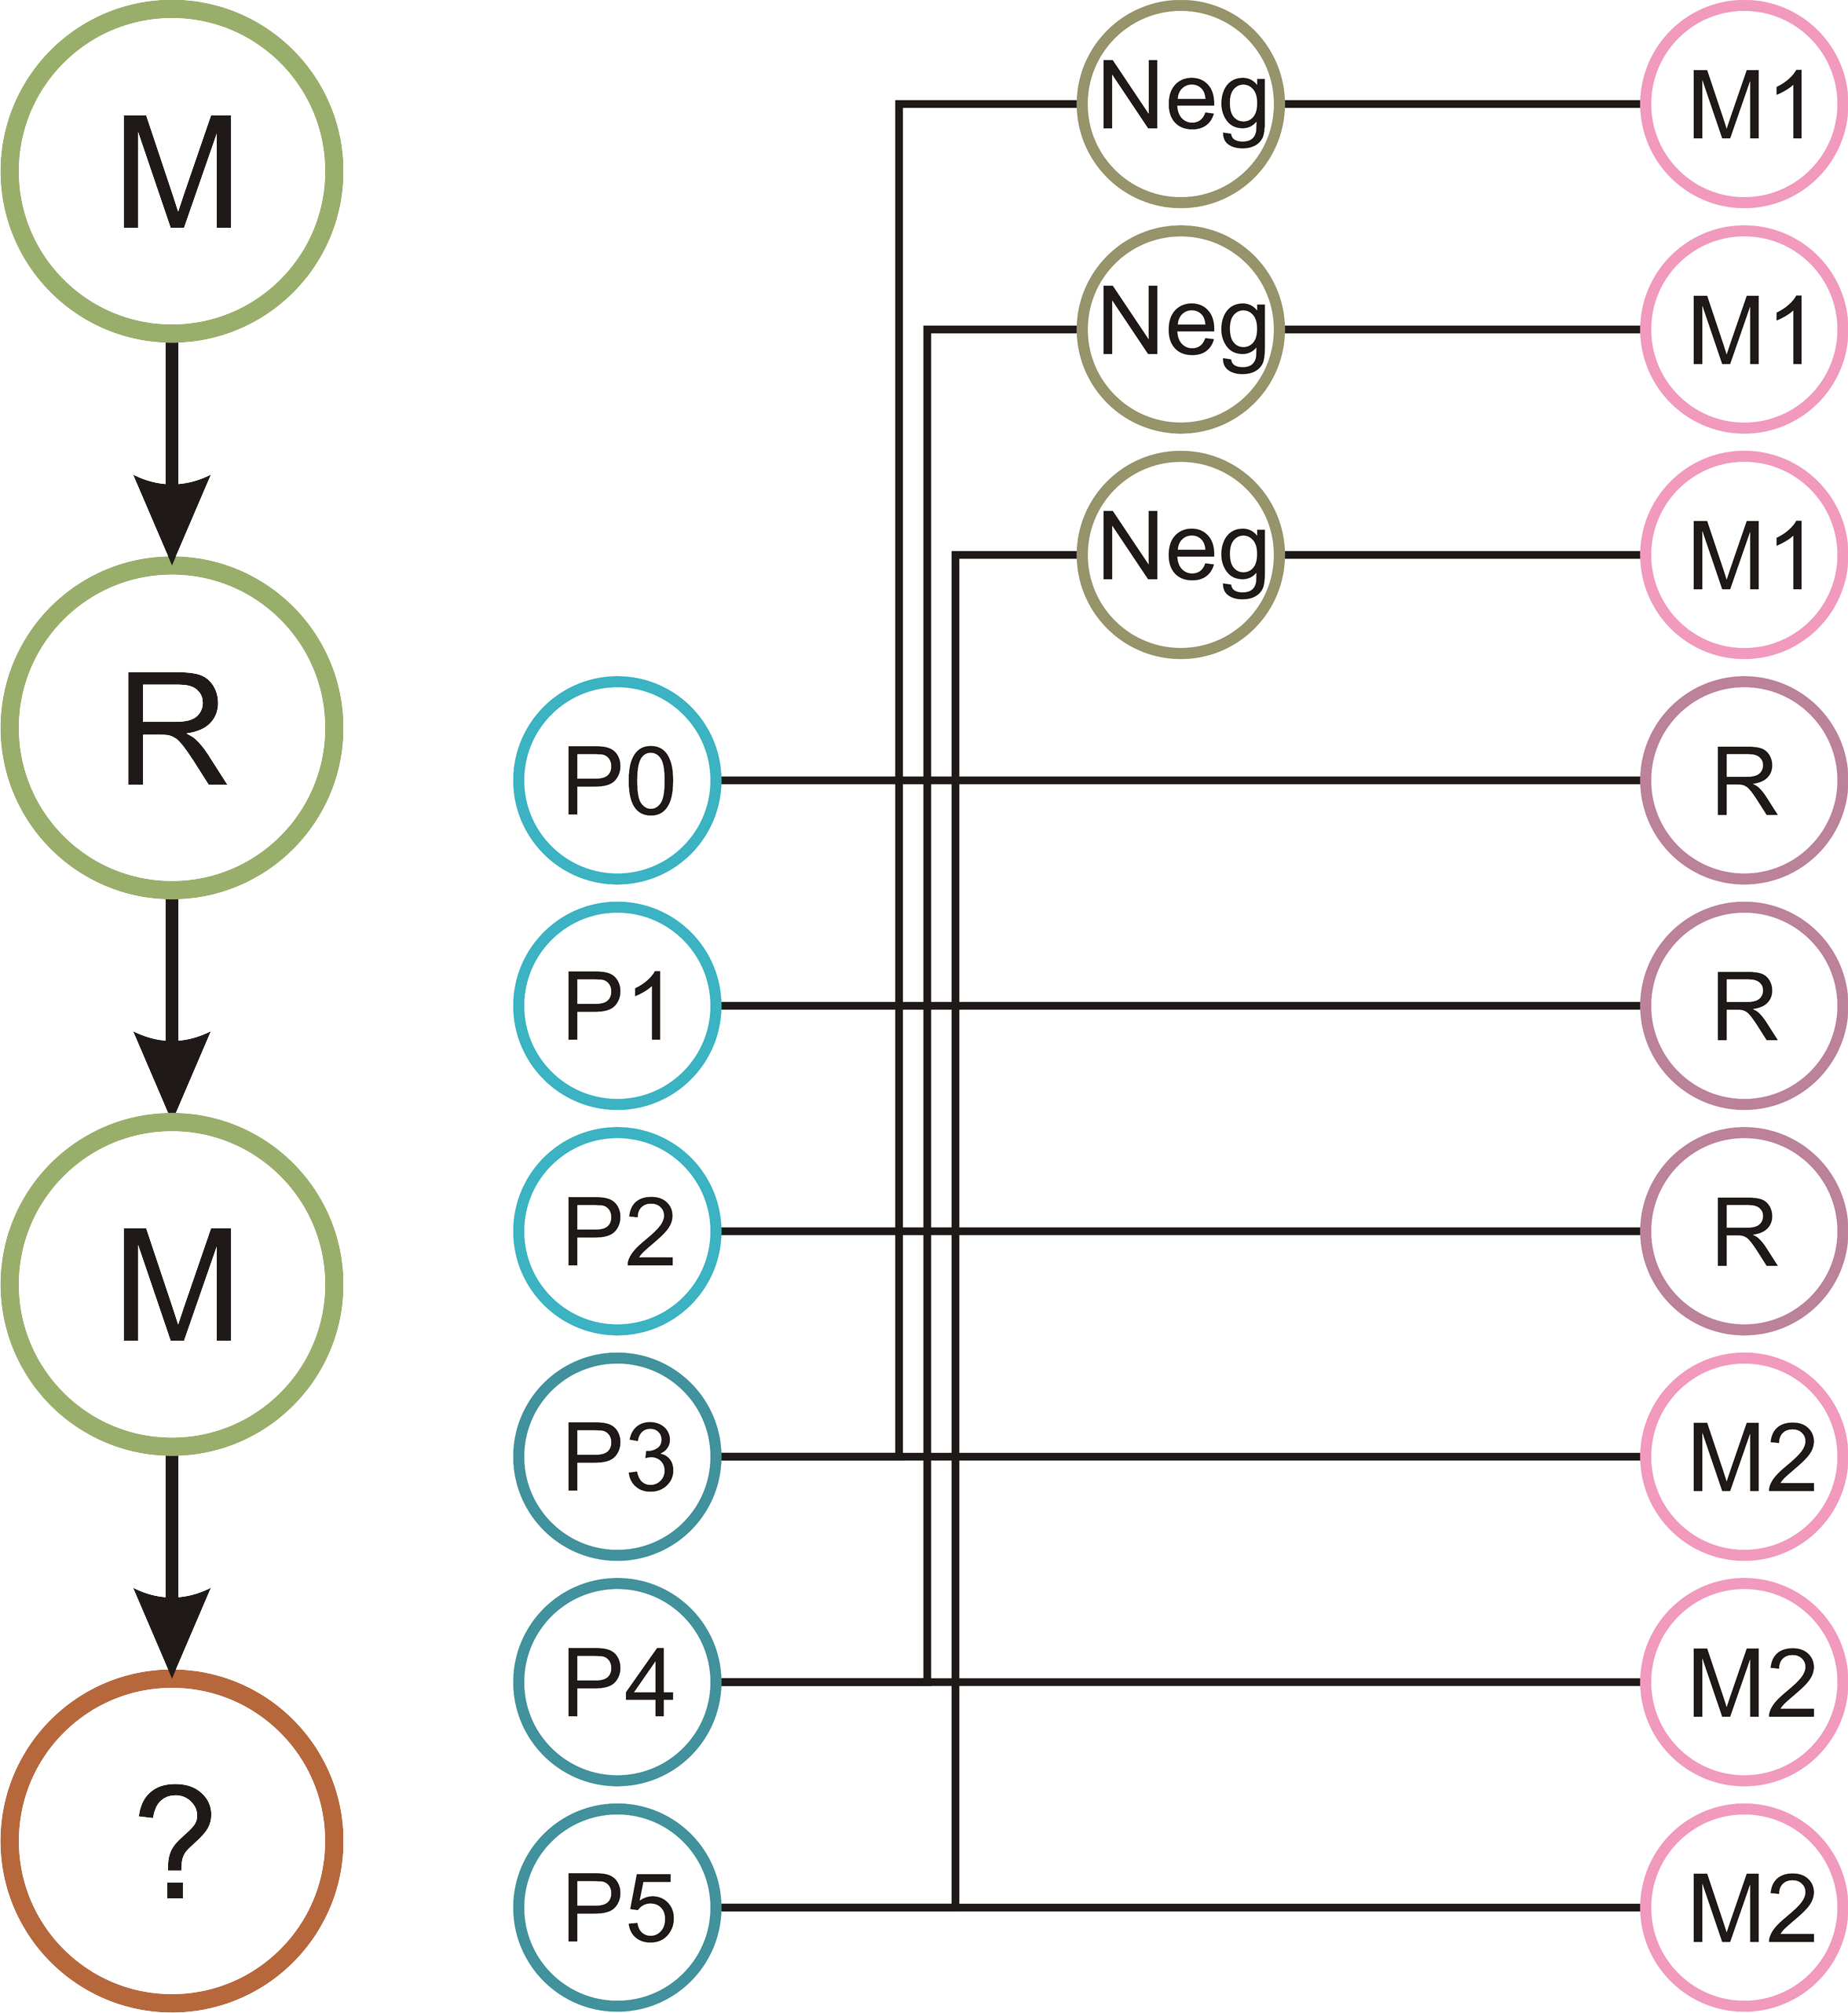
\includegraphics[width=11 cm]{graphs_crot.png}
	\caption{Слева: Поддерево узлов, реализующих сложный узел <<поворот относительно точки>>. ``R'' - узел простого поворота, ``M'' - узел перемещения, ``?'' - выход поддерева, к которому будет присоединён дочерний узел. Справа: Зависимость внутренних параметров узла <<поворот относительно точки>> от внешних. Внешние параметры $P0-P5$, графовые узлы отрицания $Neg$. Все остальные графовые узлы - внутренние параметры данного узла.}
 	\label{fig_crot}
\end{center}
\end{figure}

\par
В этих узлах, разумеется, тоже необходимо считать производные. В поддереве производные считаются также, как и обычно, но после подсчёта производных в корне поддерева, необходимо получить зависимости от внешних параметров, по зависимостям от внутренних параметров. Для этих целей граф зависимостей внутренних параметров от внешних тоже считает свою матрицу производных. Из матрицы поддерева выделяется подматрица зависимостей от внутренних параметров, и умножается на матрицу, полученную из вычислительного графа. Результат вписывается в соответствующее место незатронутой матрицы производных, и получается нужная матрица зависимостей сложного узла.
\subsubsection{Реализованный функционал}
В универсальном дифференцируемом генераторе функций расстояния со знаком уже реализовано примерно двадцать пять узлов, описывающих различные распространённые примитивы и действия над ними. Одними из первых были реализованы следующие узлы примитивов:
\begin{itemize}
    \item Шар;
    \item Параллелепипед;
    \item Цилиндр;
    \item Скруглённый параллелепипед;
    \item Призма;
    \item Конус;
\end{itemize}

\begin{figure}[H]
\begin{center}
	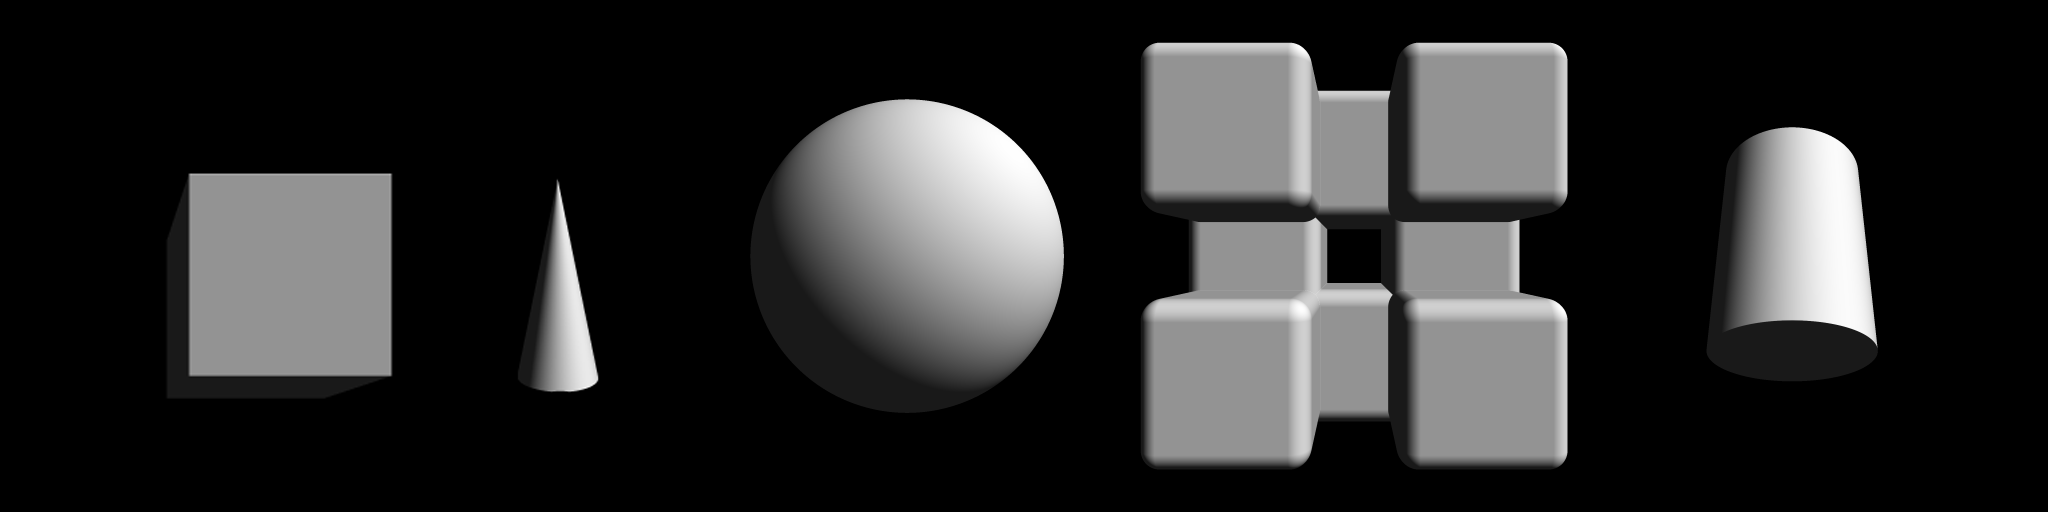
\includegraphics[width=15 cm]{primitives.png}
	\caption{Слева направо: узел - параллелепипед, узел - конус, узел - шар, комбинация нескольких узлов, каждый из которых является узлом - скруглённым параллелепипедом, повёрнутый узел - цилиндр.}
 	\label{fig_prim}
\end{center}
\end{figure}

Узлы преобразований:
\begin{itemize}
    \item Перемещение;
    \item Масштабирование;
    \item Скругление;
\end{itemize}
Узлы взаимодействий:
\begin{itemize}
    \item Объединение;
    \item Пересечение;
    \item Вычитание.
\end{itemize}

\begin{figure}[H]
\begin{center}
	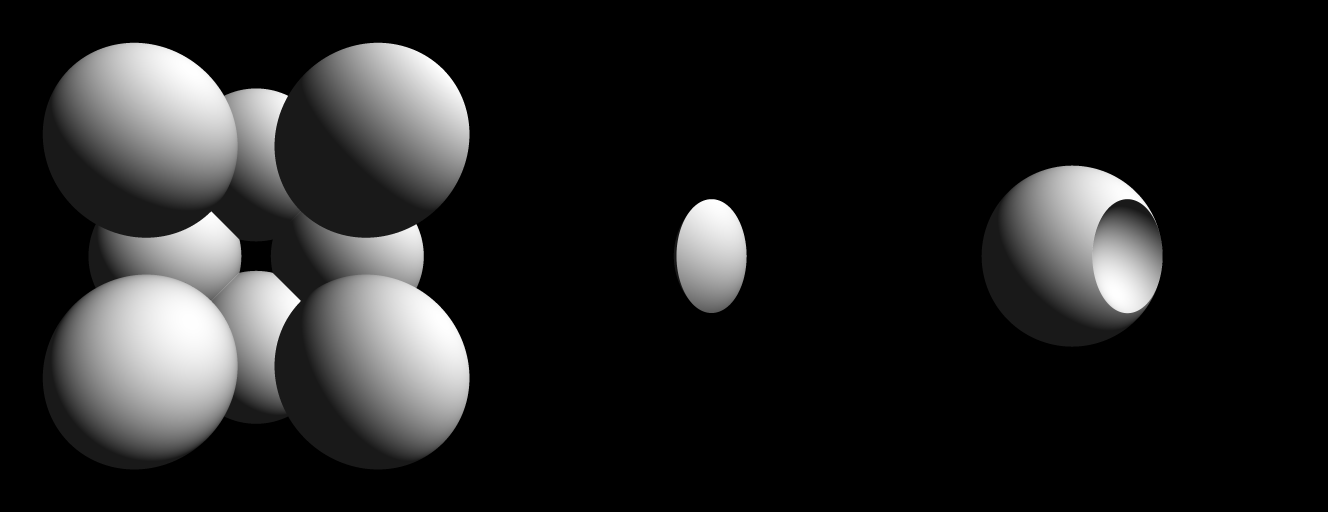
\includegraphics[width=15 cm]{combine.png}
	\caption{Слева направо: демонстрация работы узла объединение, узла пересечение, узла вычитание.}
 	\label{fig_comb}
\end{center}
\end{figure}

\par
Первым нетривиальным реализованным узлом преобразований оказался узел поворота. В нём в дочерний узел передаются изменённые параметры позиции, которые вычисляются умножением на матрицу поворота. Матрица, в свою очередь, вычисляется через три параметра: угол поворота, и два угла, задающие наклон оси вращения. Для получения производных в узле сначала вычисляются зависимости матрицы поворота от входных параметров, и через неё вычисляются необходимые производные объекта по входным параметрам, и объекта по неизменённой позиции.
\par
Следующими были реализованы несколько сложных узлов: стул и поворот относительно точки. Для них был реализован класс сложных узлов, и записаны соответствующие поддеревья и графы зависимости параметров. Их графические представления изображены на рисунках~\ref{fig_crot},~\ref{fig_chair},~\ref{fig_graph_chair}. Результат совместной работы этих узлов показан на рисунке~\ref{fig_complex}.

\begin{figure}[H]
\begin{center}
	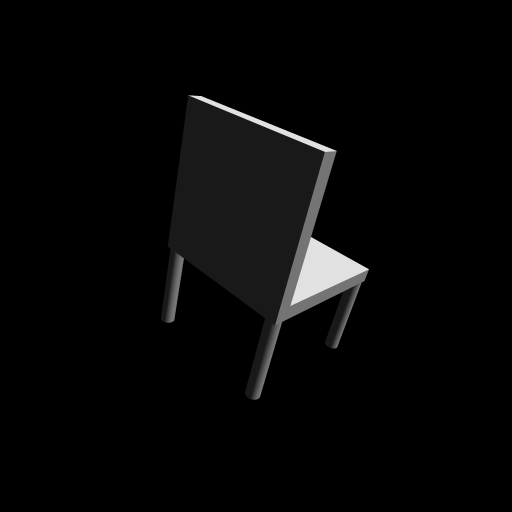
\includegraphics[width=5 cm]{complex_nodes.png}
	\caption{Сложный узел поворота относительно точки, применёный к сложному узлу <<стул>>.}
 	\label{fig_complex}
\end{center}
\end{figure}

\begin{figure}[H]
\begin{center}
	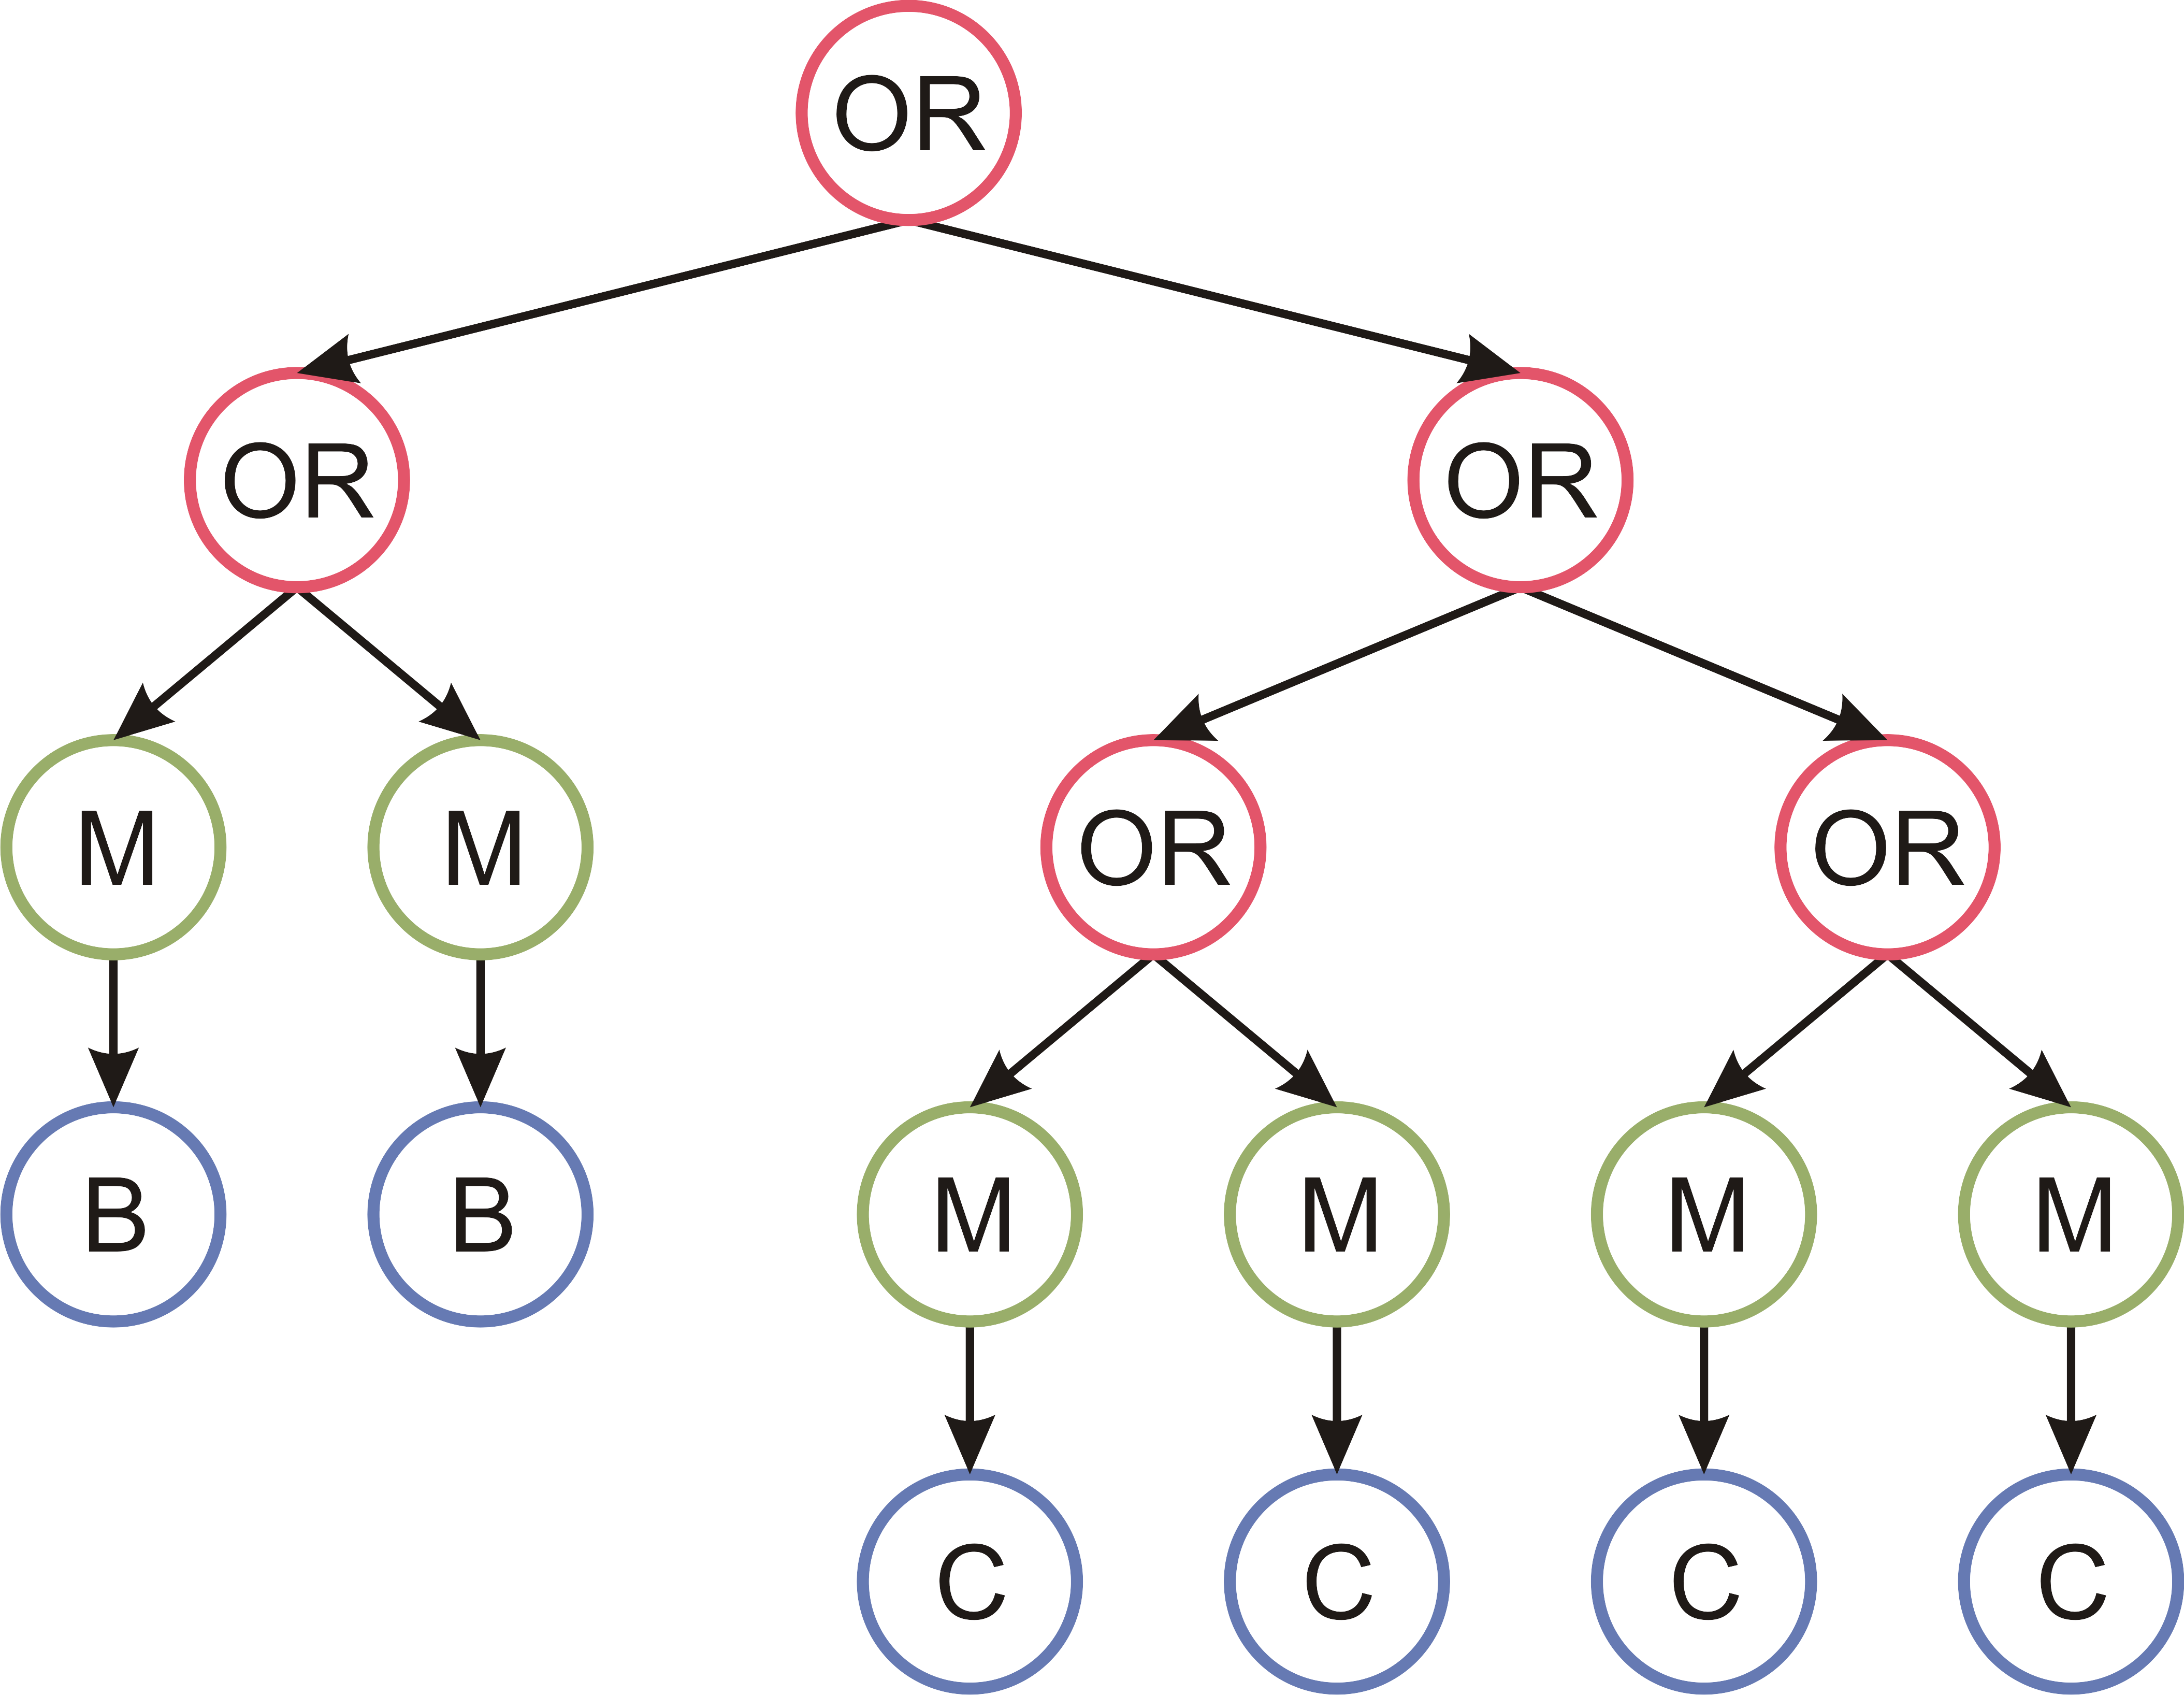
\includegraphics[width=15 cm]{chiar.png}
	\caption{Поддерево узлов, реализующих сложный узел <<стул>>. ``OR'' - узел объединения, ``M'' - узел перемещения, ``B'' - примитивный узел - параллелепипед, ``C'' - примитивный узел - цилиндр.}
 	\label{fig_chair}
\end{center}
\end{figure}

\begin{figure}[H]
\begin{center}
	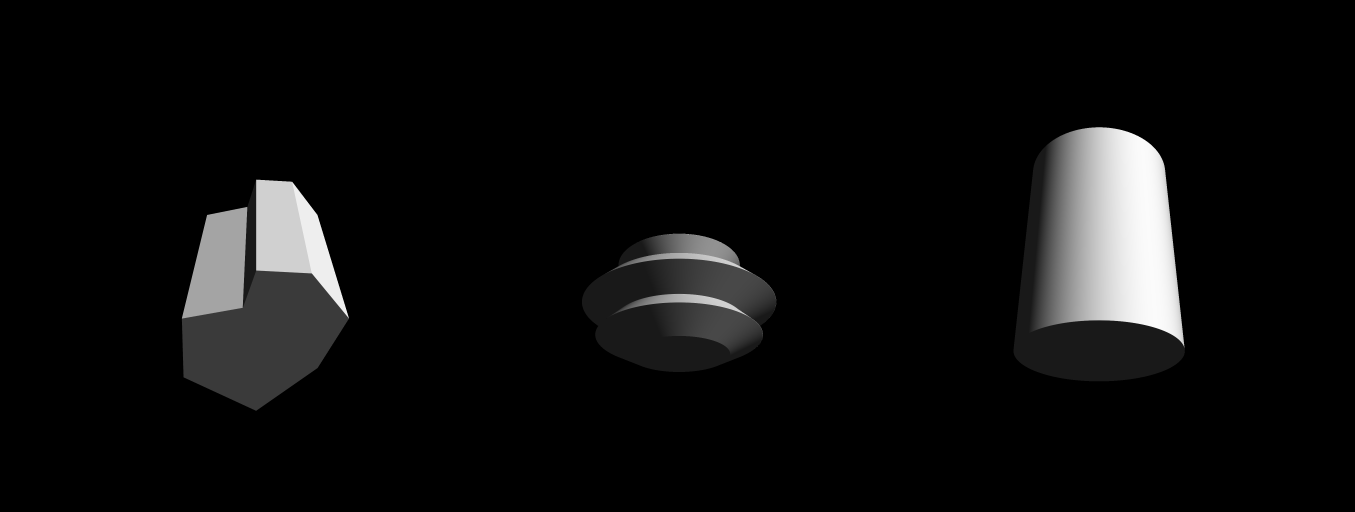
\includegraphics[width=15 cm]{extrusions_splines.png}
	\caption{Демонстрация работы, слева направо: 1) узла <<экструзии>>, применённого к узлу <<роза ветров>>, 2) узла <<тело вращения>>, 3) узла <<экструзии>>, применённого к узлу - круг (даёт результат, аналогичный использованию узла цилиндр).}
 	\label{fig_extr}
\end{center}
\end{figure}

\begin{figure}[H]
\begin{center}
	\includegraphics[width=15 cm]{graph_chair.png}
	\caption{Зависимость внутренних параметров узла <<стул>> от внешних. Внешние параметры $P0-P5$, графовые узлы вычитания $S1-S3$, графовые узлы отрицания $N1-N3$, графовый узел константа $0$. Все остальные графовые узлы - внутренние параметры данного узла.}
 	\label{fig_graph_chair}
\end{center}
\end{figure}

\par
Следующим нетривиальным узлом преобразований был узел <<экструзии>>. Это узел, который двумерный объект превращает в трёхмерный, у которого задана высота, и основание совпадает с дочерним двумерным объектом. В начале происходит проверка, откуда измеряется расстояние до объекта (сбоку от него, сверху, по диагонали, или внутри), и в зависимости от этого вычисляется результат и необходимые производные. Демонстрация работы этого узла представлены на рисунке~\ref{fig_extr}.
\par
Специально для корректного взаимодействия с узлом <<экструзии>> были созданы несколько узлов, описывающих двухмерные объекты:
\begin{itemize}
    \item Квадрат;
    \item Круг;
\end{itemize}
И взаимодействия над ними в плоскости:
\begin{itemize}
    \item Перемещение;
    \item Поворот;
    \item Поворот относительно точки.
\end{itemize}
\par
Узлы масштабирования и скругления не были переписаны для двухмерных объектов, поскольку вычисления в них и количество входных параметров полностью повторяют соответствующие им узлы преобразования в трёхмерном пространстве.
\par
Среди нетривиальных узлов также были созданы следующие узлы примитивов:
\begin{itemize}
    \item Роза ветров (полигон, задающийся точками на границах секторов);
    \item Сплайн (ломанная линия);
    \item Тело вращения (ломанная линия, повёрнутая вокруг оси).
\end{itemize}
\par
Они реализованы похожим образом, и отличаются друг от друга небольшими внутренними особенностями. Внутри каждого из них производится поиск ближайшего отрезка, относительно заданной позиции. После этого вычисляется расстояние до поверхности объекта и необходимые производные по параметрам, задающим этот отрезок, и другим, значимым для объекта. Результаты работы этих узлов представлены на изображении~\ref{fig_extr}.
\par
Узлов, которые возможно реализовать в этом универсальном генераторе, крайне много, и он легко дополняется новыми элементами. Простые узлы создаются по аналогии с уже созданными. Необходимо реализовать функцию расчёта расстояния до объекта, заданного узлом, и пересчитать матрицу производных в соответствии с формулой расстояния. При необходимости реализовать нетривиальный объект создаётся узел на основе класса сложного узла, в который записывается уникальное поддерево из уже существующих простых узлов, и необходимые взаимодействия между входными параметрами, и параметрами поддерева.

\section{Процедурная генерация в задаче реконструкции}
\subsection{Генераторы посуды и зданий}
Дифференцируемые процедурные генераторы были реализованы с целью решения задач реконструкции \cite{garifullin2023diff} \cite{garifullin2024single}. Реконструкция происходит по следующему алгоритму:
\begin{itemize}
    \item Трёхмерная модель создаётся дифференцируемым процедурным генератором;
    \item Модель вместе с параметрами сцены подаётся на вход дифференцируемому рендеру;
    \item Для выходного изображения получается силуэт объекта;
    \item Из эталонной и созданной маски вычисляется функция потерь;
    \item Проводится обратное распространение ошибки и изменяются параметры по меметическому алгоритму для следующей итерации.
\end{itemize}

\begin{figure}[H]
\begin{center}
	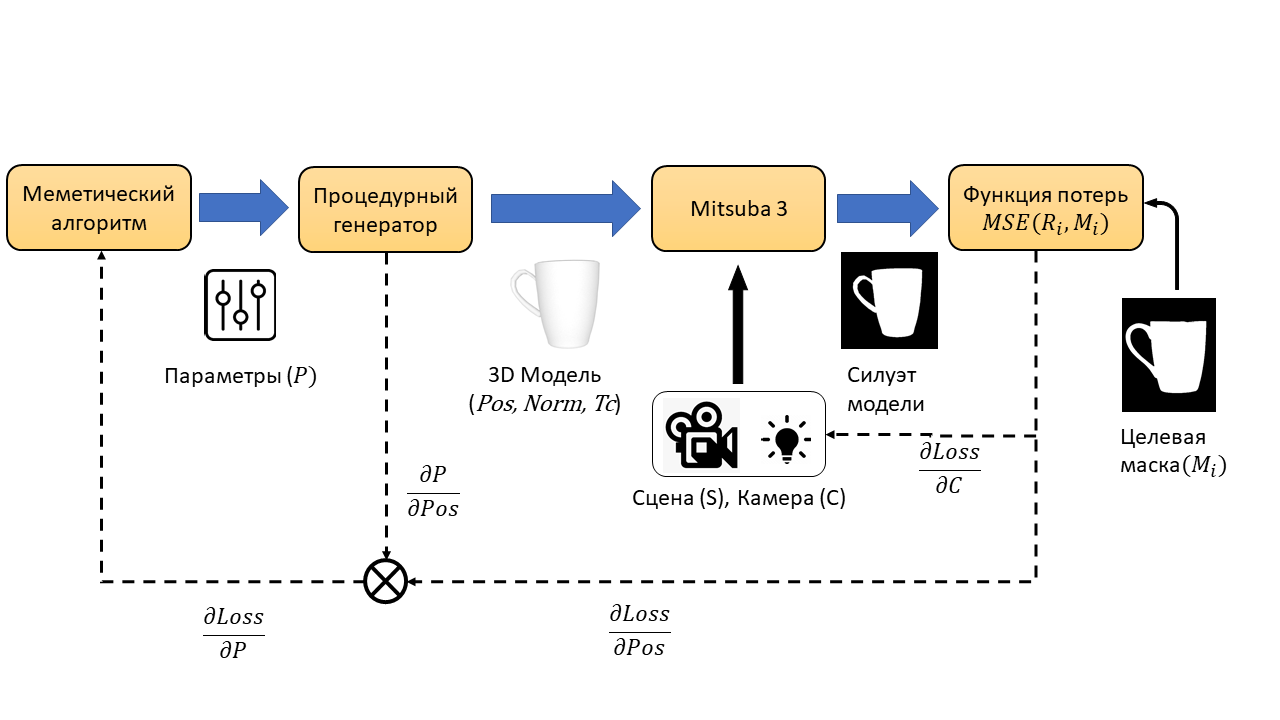
\includegraphics[width=15 cm]{pipeline.png}
	\caption{Схема метода реконструкции модели.}
 	\label{fig_reconstr}
\end{center}
\end{figure}

\par
Данный алгоритм использует дифференцируемые генераторы посуды и зданий. За счёт этого объект, полученный описанным выше методом, имеет более гладкую структуру и лучше восстанавливает форму входной модели. Процедурный генератор применяет строгие правила к структуре объекта и гарантирует, что полученная модель не будет содержать дыр, неровностей и иных геометрических артефактов, если они не предусмотрены структурой модели.

\begin{figure}[H]
\begin{center}
	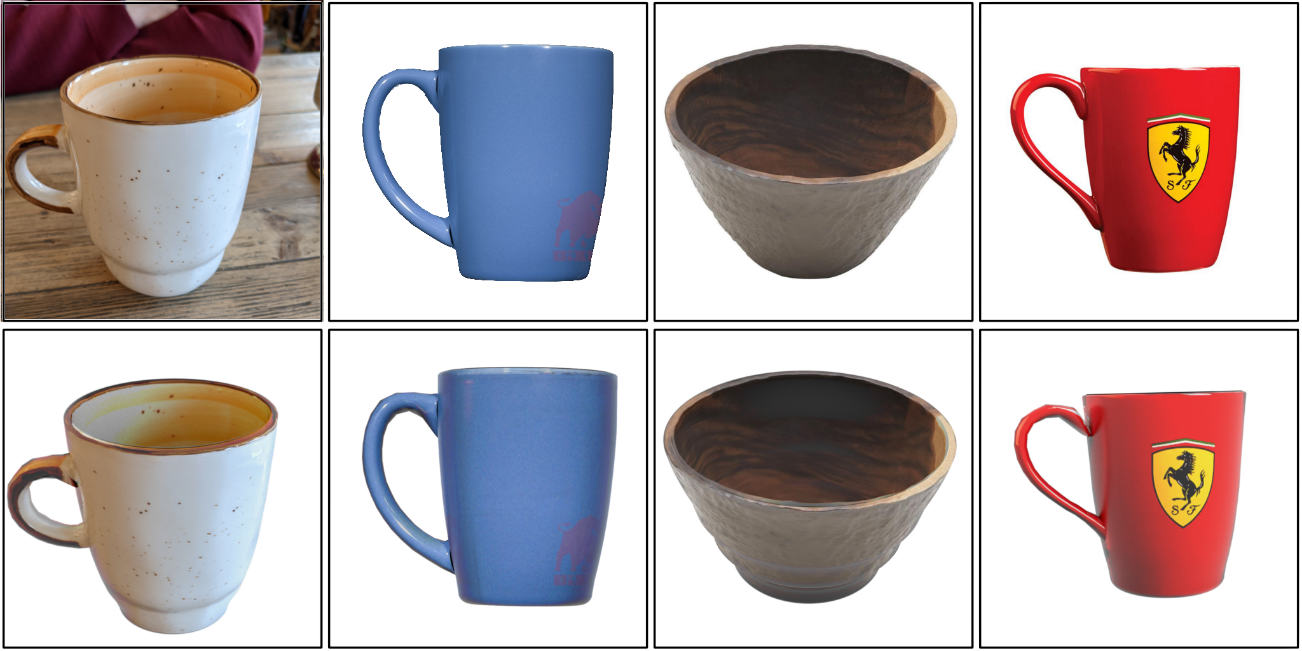
\includegraphics[width=15 cm]{results.png}
	\caption{Результаты реконструкции по одной фотографии с использованием процедурного генератора посуды. Верхний ряд: входные изображения, нижний ряд: реконструированные модели.}
 	\label{fig_dishes_r}
\end{center}
\end{figure}

\begin{figure}[H]
\begin{center}
	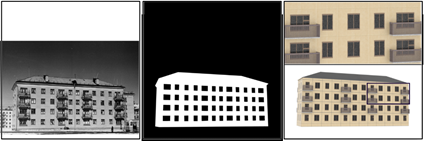
\includegraphics[width=15 cm]{houses_res.png}
	\caption{Результаты реконструкции по одной фотографии с использованием процедурного генератора зданий. Слева направо: входное изображение, маска окон, результат реконструкции с использованием текстур по умолчанию.}
 	\label{fig_houses_r}
\end{center}
\end{figure}

\par
На рисунках~\ref{fig_dishes_r} и~\ref{fig_houses_r} показаны результаты реконструкции по одному входному изображению без информации о позиции и характеристиках камеры, а также освещении. На рисунке~\ref{fig_compare} и таблице~\ref{res_table} продемонстрированно сравнение восстановления модели с использованием дифференцируемого процедурного генератора, и других методов реконструкции.
\par
\begin{figure}[H]
\begin{center}
	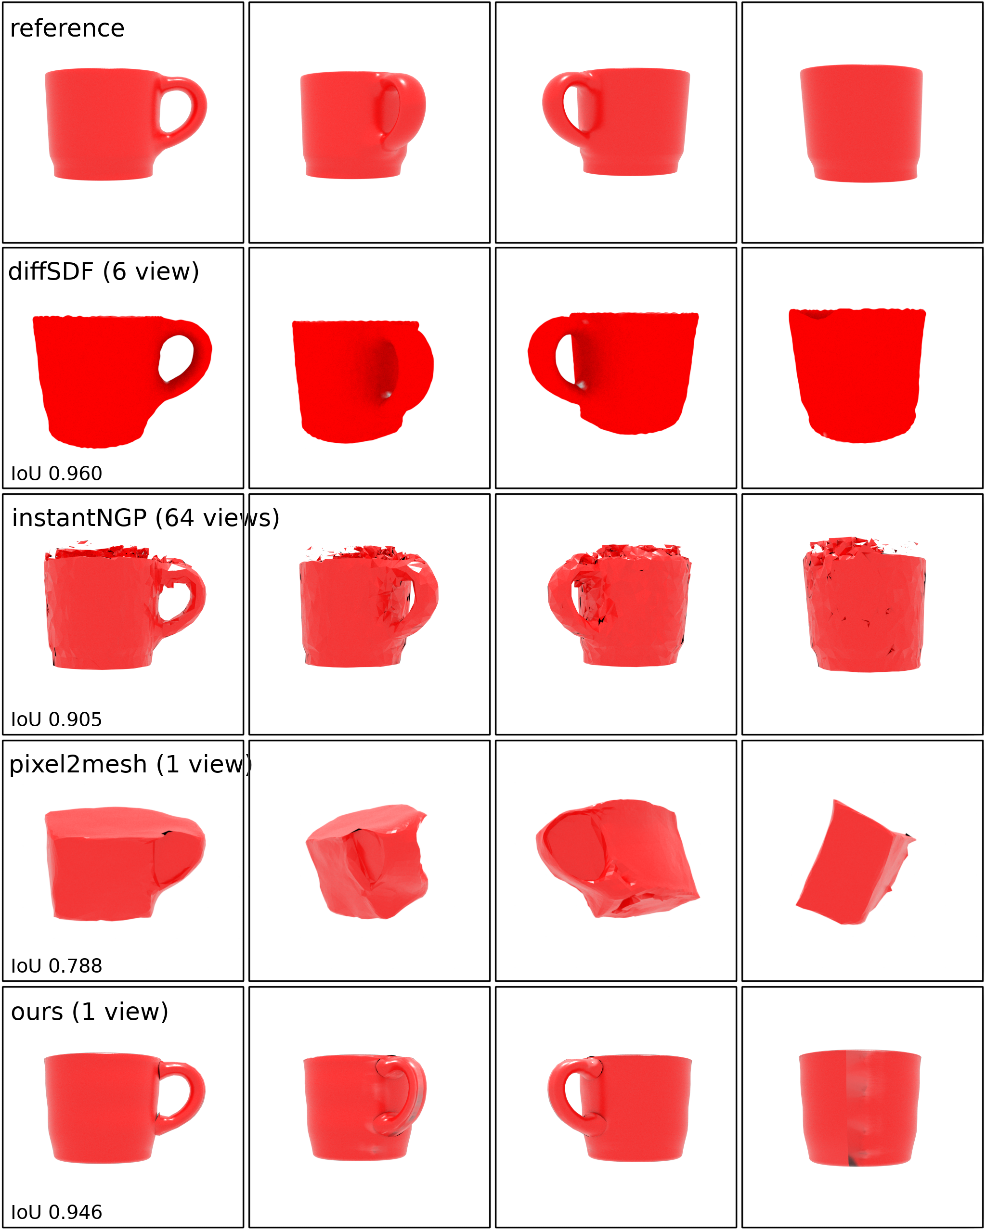
\includegraphics[width=15 cm]{checks.png}
	\caption{Сравнение результатов, полученных с использованием данного метода, с дифференцируемой реконструкцией SDF \cite{vicini2022differentiable}, InstantNGP \cite{muller2022instant} и Pixel2Mesh \cite{wang2018pixel2mesh}.}
 	\label{fig_compare}
\end{center}
\end{figure}

\begin{figure}[H]
\begin{center}
	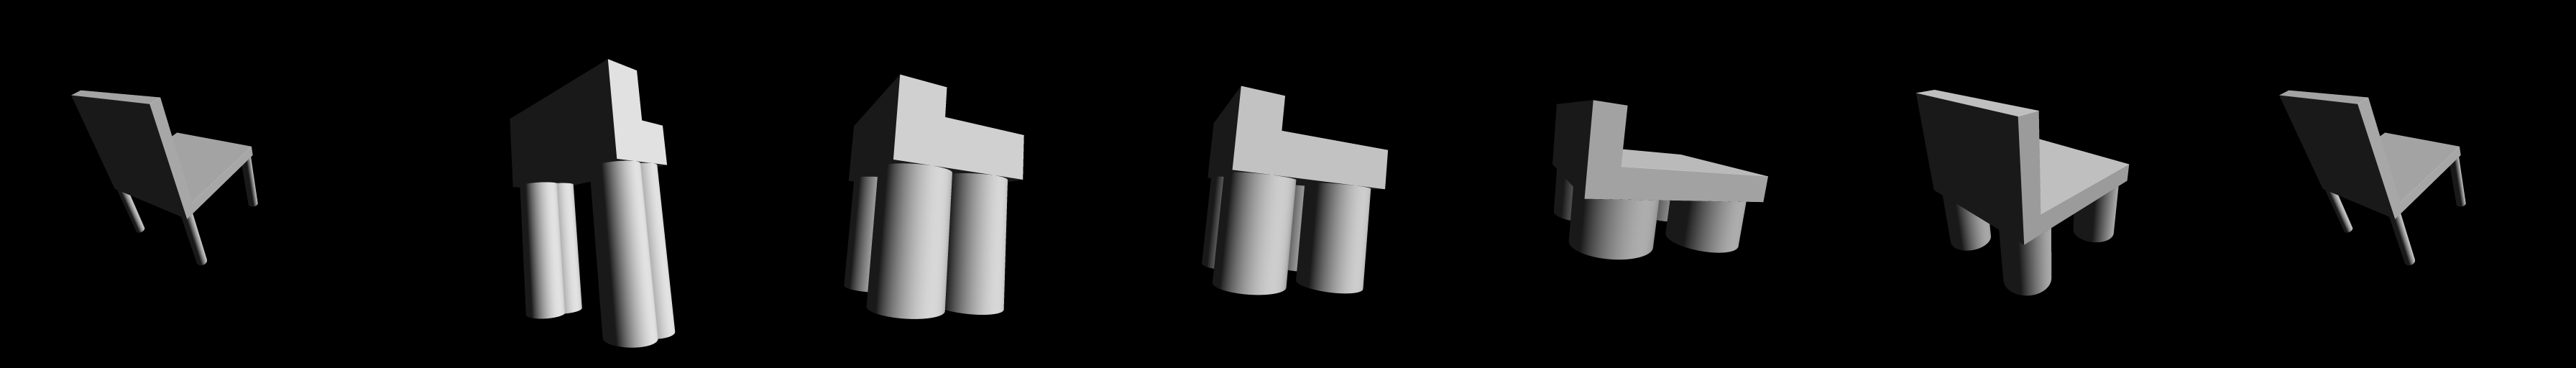
\includegraphics[width=15 cm]{chair_optimization.png}
	\caption{Слева направо: целевая модель, исходная модель, модель после 100 итераций градиентного спуска, 200 итераций, 500 итераций, 750 итераций, оптимизированная модель (1000 итераций)}
 	\label{fig_chair_opt}
\end{center}
\end{figure}

\begin{table}[H] 
	\begin{tabularx}{\textwidth}{cccc}
		\toprule
		\textbf{Алгоритм}	& \textbf{cup\_1}	& \textbf{cup\_2} & \textbf{building}\\
		\midrule
		DiffSDF (2 изображения) 		& 0.787 & 0.422 & 0.728\\
		DiffSDF (6 изображений) 		& 0.960 & 0.502 & \textbf{0.967}\\
		DiffSDF (12 изображений) 		& \textbf{0.984} & 0.669 & \textbf{0.979}\\
		InstantNGP (16 изображений) 	& 0.858 & 0.878 & 0.940\\
		InstantNGP (64 изображения) 	& 0.905 & 0.930 & 0.971\\
		Pixel2Mesh (1 изображение)     & 0.788 & 0.513 & 0.626\\
		TGS (1 изображение)        	& 0.939 & 0.925 & 0.965\\
		Предложенный метод (1 изображение)	& 0.948 & 0.972 & 0.886\\
		Предложенный метод (2 изображения)	& 0.951 & \textbf{0.978} & 0.890\\
		Предложенный метод (4 изображения)	& \textbf{0.962} & \textbf{0.979} & 0.869\\
		\bottomrule
	\end{tabularx}
 \caption{Среднее значение IoU (больше - лучше) для различных моделей.}\label{res_table}
\end{table}

\subsection{Универсальный генератор}
Универсальный дифференцируемый процедурный генератор также может использоваться в задачах реконструкции трёхмерных объектов. При использовании фиксированного заранее заданного дерева генератора, объекты соответствующего класса могут восстанавливаться по схожему с выше изложенным алгоритму. На рисунке~\ref{fig_chair_opt} проиллюстрирован процесс оптимизации модели градиентным спуском с фиксированным деревом.
\par
В этом случае генератор не используется как универсальный. Оптимальным бы являлось использовать получать модели при помощи генератора, не зависимо от их класса, и без выбора одного конкретного дерева внутри него. В этом и состоит главная сложность создания универсального алгоритма реконструкции, что восстанавливаться должен не только объект, но и структура генератора. Но потенциал у использования универсального дифференцируемого генератора в задаче реконструкции есть. При его успешной реализации, художники и 3D моделисты смогут легко получать начальное приближение необходимого объекта и просто модифицировать структуру генератора или полученные параметры модели.
\par

Произвести сравнение реализованных генераторов с другими обратными процедурными генераторами по какой-либо метрике не представляется целесообразным. Однако, можно попробовать сравнить важные в контексте данной работы характеристики некоторых обратных генераторов. В задаче трёхмерной реконструкции с использованием метода, представленного ранее, генератор должен быть дифференцируемым. Для реконструкции разных моделей, генератор должен восстанавливать как можно большее количество классов объектов, а в идеале быть универсальным. Данное сравнение продемонстрированно в таблице~\ref{comp_table}.

\begin{table}[H] 
	\begin{tabularx}{\textwidth}{cccc}
		\toprule
		\textbf{Алгоритм}	& \textbf{Классы}	& \textbf{Дискр. пар.} & \textbf{Дифф.}\\
		\midrule
		Proc. Architectural Models \cite{urban1} 		& Здания & \textbf{+} & \textbf{-}\\
		Inv. Proc. Mod. of L-systems \cite{vst2010inverse} 	& 2D изображения & \textbf{+} & \textbf{-}\\
		Inv. Proc. Mod. of Branching Structures \cite{guo2020inverse} 	& 2D изображения & \textbf{+} & \textbf{-}\\
		Inv. Proc. Mod. of Trees \cite{stava2014inverse}     & Деревья & \textbf{+} & \textbf{-}\\
		Proc. Mod. of Buildings \cite{muller2006procedural}      & Здания & \textbf{+} & \textbf{-}\\
		Предложенный метод тип 1	& Посуда & \textbf{+} & \textbf{+}\\
		Предложенный метод тип 2	& Здания & \textbf{+} & \textbf{+}\\
		Предложенный метод универсальный	& Любые & \textbf{+} & \textbf{+}\\
		\bottomrule
	\end{tabularx}
 \caption{Важные характеристики разных процедурных генераторов. (Генерируемые классы объектов, Наличие дискретных параметров, Дифференцируемость)}\label{comp_table}
\end{table}

\section{Заключение}
Данная работа посвящена созданию дифференцируемых процедурных генераторов, и реализации составляющих универсального дифференцируемого процедурного генератора 3D моделей. Дифференцируемость генераторов была использована в задаче трёхмерной реконструкции, а полученные результаты были проанализированы.
\par
В рамках данной работы:
\begin{itemize}
    \item Были реализованы дифференцируемые процедурные генераторы двух классов объектов, а конкретно, посуды и зданий;
    \item Генераторы были успешно интегрированы в программу 3D реконструкции;
    \item Результаты реконструкции, полученные с использованием дифференцируемых процедурных генераторов, были получены и произведена экспериментальная оценка;
    \item Также были разработаны составляющие универсальных дифференцируемых процедурных генераторов, с возможностью их дальнейшей модификации, использующих представления объектов как полигональные сетки, и как функции расстояния со знаком.
\end{itemize}
\par
Результаты, полученные после интеграции генераторов в программу для реконструкции, были описаны в статье \cite{garifullin2023diff} \cite{garifullin2024single}, представленной на международной конференции ГрафиКон 2023 года и опубликованной в Q1 журнале “Symmetry”.


\newpage
\bibliographystyle{unsrt}
\bibliography{biblio}
\end{document}